%%
% Copyright (c) 2017 - 2026, Pascal Wagler;
% Copyright (c) 2014 - 2026, John MacFarlane
%
% All rights reserved.
%
% Redistribution and use in source and binary forms, with or without
% modification, are permitted provided that the following conditions
% are met:
%
% - Redistributions of source code must retain the above copyright
% notice, this list of conditions and the following disclaimer.
%
% - Redistributions in binary form must reproduce the above copyright
% notice, this list of conditions and the following disclaimer in the
% documentation and/or other materials provided with the distribution.
%
% - Neither the name of John MacFarlane nor the names of other
% contributors may be used to endorse or promote products derived
% from this software without specific prior written permission.
%
% THIS SOFTWARE IS PROVIDED BY THE COPYRIGHT HOLDERS AND CONTRIBUTORS
% "AS IS" AND ANY EXPRESS OR IMPLIED WARRANTIES, INCLUDING, BUT NOT
% LIMITED TO, THE IMPLIED WARRANTIES OF MERCHANTABILITY AND FITNESS
% FOR A PARTICULAR PURPOSE ARE DISCLAIMED. IN NO EVENT SHALL THE
% COPYRIGHT OWNER OR CONTRIBUTORS BE LIABLE FOR ANY DIRECT, INDIRECT,
% INCIDENTAL, SPECIAL, EXEMPLARY, OR CONSEQUENTIAL DAMAGES (INCLUDING,
% BUT NOT LIMITED TO, PROCUREMENT OF SUBSTITUTE GOODS OR SERVICES;
% LOSS OF USE, DATA, OR PROFITS; OR BUSINESS INTERRUPTION) HOWEVER
% CAUSED AND ON ANY THEORY OF LIABILITY, WHETHER IN CONTRACT, STRICT
% LIABILITY, OR TORT (INCLUDING NEGLIGENCE OR OTHERWISE) ARISING IN
% ANY WAY OUT OF THE USE OF THIS SOFTWARE, EVEN IF ADVISED OF THE
% POSSIBILITY OF SUCH DAMAGE.
%%

%%
% This is the Eisvogel pandoc LaTeX template.
%
% For usage information and examples visit the official GitHub page:
% https://github.com/Wandmalfarbe/pandoc-latex-template
%%
% Options for packages loaded elsewhere
\PassOptionsToPackage{unicode}{hyperref}
\PassOptionsToPackage{hyphens}{url}
\PassOptionsToPackage{dvipsnames,svgnames,x11names,table}{xcolor}
\documentclass[
  11pt,
  paper=a4,
  ,captions=tableheading
]{scrartcl}
\usepackage{xcolor}
\usepackage[margin=1in]{geometry}
\usepackage{amsmath,amssymb}

% add backlinks to footnote references, cf. https://tex.stackexchange.com/questions/302266/make-footnote-clickable-both-ways
\usepackage{footnotebackref}
\setcounter{secnumdepth}{-\maxdimen} % remove section numbering
\usepackage{iftex}
\ifPDFTeX
  \usepackage[T1]{fontenc}
  \usepackage[utf8]{inputenc}
  \usepackage{textcomp} % provide euro and other symbols
\else % if luatex or xetex
  \usepackage{unicode-math} % this also loads fontspec
  \defaultfontfeatures{Scale=MatchLowercase}
  \defaultfontfeatures[\rmfamily]{Ligatures=TeX,Scale=1}
\fi
\usepackage{lmodern}
\ifPDFTeX\else
  % xetex/luatex font selection
  \setmainfont[]{Helvetica}
  \setmonofont[]{Menlo}
\fi
% Use upquote if available, for straight quotes in verbatim environments
\IfFileExists{upquote.sty}{\usepackage{upquote}}{}
\IfFileExists{microtype.sty}{% use microtype if available
  \usepackage[]{microtype}
  \UseMicrotypeSet[protrusion]{basicmath} % disable protrusion for tt fonts
}{}

% Use setspace anyway because we change the default line spacing.
% The spacing is changed early to affect the titlepage and the TOC.
\usepackage{setspace}
\setstretch{1.2}
\makeatletter
\@ifundefined{KOMAClassName}{% if non-KOMA class
  \IfFileExists{parskip.sty}{%
    \usepackage{parskip}
  }{% else
    \setlength{\parindent}{0pt}
    \setlength{\parskip}{6pt plus 2pt minus 1pt}}
}{% if KOMA class
  \KOMAoptions{parskip=half}}
\makeatother
\usepackage{etoolbox}
\BeforeBeginEnvironment{lstlisting}{\par\noindent\begin{minipage}{\linewidth}}
\AfterEndEnvironment{lstlisting}{\end{minipage}\par\addvspace{\topskip}}
\usepackage{color}
\usepackage{fancyvrb}
\newcommand{\VerbBar}{|}
\newcommand{\VERB}{\Verb[commandchars=\\\{\}]}
\DefineVerbatimEnvironment{Highlighting}{Verbatim}{commandchars=\\\{\}}
% Add ',fontsize=\small' for more characters per line
\newenvironment{Shaded}{}{}
\newcommand{\AlertTok}[1]{\textcolor[rgb]{1.00,0.00,0.00}{\textbf{#1}}}
\newcommand{\AnnotationTok}[1]{\textcolor[rgb]{0.38,0.63,0.69}{\textbf{\textit{#1}}}}
\newcommand{\AttributeTok}[1]{\textcolor[rgb]{0.49,0.56,0.16}{#1}}
\newcommand{\BaseNTok}[1]{\textcolor[rgb]{0.25,0.63,0.44}{#1}}
\newcommand{\BuiltInTok}[1]{\textcolor[rgb]{0.00,0.50,0.00}{#1}}
\newcommand{\CharTok}[1]{\textcolor[rgb]{0.25,0.44,0.63}{#1}}
\newcommand{\CommentTok}[1]{\textcolor[rgb]{0.38,0.63,0.69}{\textit{#1}}}
\newcommand{\CommentVarTok}[1]{\textcolor[rgb]{0.38,0.63,0.69}{\textbf{\textit{#1}}}}
\newcommand{\ConstantTok}[1]{\textcolor[rgb]{0.53,0.00,0.00}{#1}}
\newcommand{\ControlFlowTok}[1]{\textcolor[rgb]{0.00,0.44,0.13}{\textbf{#1}}}
\newcommand{\DataTypeTok}[1]{\textcolor[rgb]{0.56,0.13,0.00}{#1}}
\newcommand{\DecValTok}[1]{\textcolor[rgb]{0.25,0.63,0.44}{#1}}
\newcommand{\DocumentationTok}[1]{\textcolor[rgb]{0.73,0.13,0.13}{\textit{#1}}}
\newcommand{\ErrorTok}[1]{\textcolor[rgb]{1.00,0.00,0.00}{\textbf{#1}}}
\newcommand{\ExtensionTok}[1]{#1}
\newcommand{\FloatTok}[1]{\textcolor[rgb]{0.25,0.63,0.44}{#1}}
\newcommand{\FunctionTok}[1]{\textcolor[rgb]{0.02,0.16,0.49}{#1}}
\newcommand{\ImportTok}[1]{\textcolor[rgb]{0.00,0.50,0.00}{\textbf{#1}}}
\newcommand{\InformationTok}[1]{\textcolor[rgb]{0.38,0.63,0.69}{\textbf{\textit{#1}}}}
\newcommand{\KeywordTok}[1]{\textcolor[rgb]{0.00,0.44,0.13}{\textbf{#1}}}
\newcommand{\NormalTok}[1]{#1}
\newcommand{\OperatorTok}[1]{\textcolor[rgb]{0.40,0.40,0.40}{#1}}
\newcommand{\OtherTok}[1]{\textcolor[rgb]{0.00,0.44,0.13}{#1}}
\newcommand{\PreprocessorTok}[1]{\textcolor[rgb]{0.74,0.48,0.00}{#1}}
\newcommand{\RegionMarkerTok}[1]{#1}
\newcommand{\SpecialCharTok}[1]{\textcolor[rgb]{0.25,0.44,0.63}{#1}}
\newcommand{\SpecialStringTok}[1]{\textcolor[rgb]{0.73,0.40,0.53}{#1}}
\newcommand{\StringTok}[1]{\textcolor[rgb]{0.25,0.44,0.63}{#1}}
\newcommand{\VariableTok}[1]{\textcolor[rgb]{0.10,0.09,0.49}{#1}}
\newcommand{\VerbatimStringTok}[1]{\textcolor[rgb]{0.25,0.44,0.63}{#1}}
\newcommand{\WarningTok}[1]{\textcolor[rgb]{0.38,0.63,0.69}{\textbf{\textit{#1}}}}

% Workaround/bugfix from jannick0.
% See https://github.com/jgm/pandoc/issues/4302#issuecomment-360669013)
% or https://github.com/Wandmalfarbe/pandoc-latex-template/issues/2
%
% Redefine the verbatim environment 'Highlighting' to break long lines (with
% the help of fvextra). Redefinition is necessary because it is unlikely that
% pandoc includes fvextra in the default template.
\usepackage{fvextra}
\DefineVerbatimEnvironment{Highlighting}{Verbatim}{breaklines,fontsize=\scriptsize,commandchars=\\\{\}}

\usepackage{longtable,booktabs,array}
\newcounter{none} % for unnumbered tables
\usepackage{calc} % for calculating minipage widths
% Correct order of tables after \paragraph or \subparagraph
\usepackage{etoolbox}
\makeatletter
\patchcmd\longtable{\par}{\if@noskipsec\mbox{}\fi\par}{}{}
\makeatother
% Allow footnotes in longtable head/foot
\IfFileExists{footnotehyper.sty}{\usepackage{footnotehyper}}{\usepackage{footnote}}
\usepackage{graphicx}
\makeatletter
\newsavebox\pandoc@box
\newcommand*\pandocbounded[1]{% scales image to fit in text height/width
  \sbox\pandoc@box{#1}%
  \Gscale@div\@tempa{\textheight}{\dimexpr\ht\pandoc@box+\dp\pandoc@box\relax}%
  \Gscale@div\@tempb{\linewidth}{\wd\pandoc@box}%
  \ifdim\@tempb\p@<\@tempa\p@\let\@tempa\@tempb\fi% select the smaller of both
  \ifdim\@tempa\p@<\p@\scalebox{\@tempa}{\usebox\pandoc@box}%
  \else\usebox{\pandoc@box}%
  \fi%
}
% Set default figure placement to htbp
% Make use of float-package and set default placement for figures to H.
% The option H means 'PUT IT HERE' (as  opposed to the standard h option which means 'You may put it here if you like').
\usepackage{float}
\floatplacement{figure}{H}
\makeatother
\setlength{\emergencystretch}{3em} % prevent overfull lines
\providecommand{\tightlist}{%
  \setlength{\itemsep}{0pt}\setlength{\parskip}{0pt}}
\usepackage{bookmark}
\IfFileExists{xurl.sty}{\usepackage{xurl}}{} % add URL line breaks if available
\urlstyle{same}
\definecolor{default-linkcolor}{HTML}{A50000}
\definecolor{default-filecolor}{HTML}{A50000}
\definecolor{default-citecolor}{HTML}{4077C0}
\definecolor{default-urlcolor}{HTML}{4077C0}

\hypersetup{
  pdftitle={GCF: A Token-Optimized Wire Format for Structured LLM Interactions},
  pdfauthor={Dayna Blackwell, Blackwell Systems},
  colorlinks=true,
  linkcolor={blue},
  filecolor={default-filecolor},
  citecolor={default-citecolor},
  urlcolor={blue},
  breaklinks=true,
  pdfcreator={LaTeX via pandoc with the Eisvogel template}}

\title{GCF: A Token-Optimized Wire Format for Structured LLM
Interactions}
\author{Dayna Blackwell, Blackwell Systems}
\date{2026-06-06 · DOI: 10.5281/zenodo.20579817}


%
% for the background color of the title page
%
\usepackage{pagecolor}
\usepackage{afterpage}

%
% break urls
%
\PassOptionsToPackage{hyphens}{url}

%
% When using babel or polyglossia with biblatex, loading csquotes is recommended
% to ensure that quoted texts are typeset according to the rules of your main language.
%
\usepackage{csquotes}

%
% captions
%
\definecolor{caption-color}{HTML}{777777}
\usepackage[font={stretch=1.2}, textfont={color=caption-color}, position=top, skip=4mm, labelfont=bf, singlelinecheck=false, justification=raggedright]{caption}
\setcapindent{0em}

%
% blockquote
%
\definecolor{blockquote-border}{RGB}{221,221,221}
\definecolor{blockquote-text}{RGB}{119,119,119}
\usepackage{mdframed}
\newmdenv[rightline=false,bottomline=false,topline=false,linewidth=3pt,linecolor=blockquote-border,skipabove=\parskip]{customblockquote}
\renewenvironment{quote}{\begin{customblockquote}\list{}{\rightmargin=0em\leftmargin=0em}%
\item\relax\color{blockquote-text}\ignorespaces}{\unskip\unskip\endlist\end{customblockquote}}

%
% Source Sans Pro as the default font family
% Source Code Pro for monospace text
%
% 'default' option sets the default
% font family to Source Sans Pro, not \sfdefault.
%
% Note that the font has been officially renamed to `Source Sans 3`, and
% You can install the newer version locally and use it, for example, with
% `mainfont: "Source Sans 3"` in the YAML metadata (requires XeTeX or LuaTeX).
%
\ifnum 0\ifxetex 1\fi\ifluatex 1\fi=0 % if pdftex
  \else % if not pdftex
    \fi

%
% heading color
%
\definecolor{heading-color}{RGB}{40,40,40}
% By default, the KOMA-Script classes will typeset sectioning headings in
% sans-serif. Use the normal body font for headings.
\addtokomafont{disposition}{\normalfont\color{heading-color}\bfseries}

%
% variables for title, author and date
%
\usepackage{titling}
\title{GCF: A Token-Optimized Wire Format for Structured LLM
Interactions}
\author{Dayna Blackwell, Blackwell Systems}
\date{2026-06-06 · DOI: 10.5281/zenodo.20579817}

%
% tables
%

\definecolor{table-row-color}{HTML}{F5F5F5}
\definecolor{table-rule-color}{HTML}{999999}

%\arrayrulecolor{black!40}
\arrayrulecolor{table-rule-color}     % color of \toprule, \midrule, \bottomrule
\setlength\heavyrulewidth{0.3ex}      % thickness of \toprule, \bottomrule
\renewcommand{\arraystretch}{1.3}     % spacing (padding)


%
% remove paragraph indentation
%
\setlength{\parindent}{0pt}
\setlength{\parskip}{6pt plus 2pt minus 1pt}
\setlength{\emergencystretch}{3em}  % prevent overfull lines

%
%
% Listings
%
%


%
% header and footer
%
\usepackage[headsepline,footsepline]{scrlayer-scrpage}

\newpairofpagestyles{eisvogel-header-footer}{
  \clearpairofpagestyles
  \ihead*{GCF Whitepaper}
  \chead*{}
  \ohead*{Blackwell Systems}
  \ifoot*{gcformat.com}
  \cfoot*{}
  \ofoot*{\thepage}
  \addtokomafont{pageheadfoot}{\upshape}
}
\pagestyle{eisvogel-header-footer}



%
% Define watermark
%

\begin{document}

\begin{titlepage}
\newgeometry{left=6cm}
\definecolor{titlepage-color}{HTML}{0a0a0a}
\newpagecolor{titlepage-color}\afterpage{\restorepagecolor}
\newcommand{\colorRule}[3][black]{\textcolor[HTML]{#1}{\rule{#2}{#3}}}
\begin{flushleft}
\noindent
\\[-1em]
\color[HTML]{ffffff}
\makebox[0pt][l]{\colorRule[2563eb]{1.3\textwidth}{4pt}}
\par
\noindent

{
  \setstretch{1.4}
  \vfill
  \noindent {\huge \textbf{\textsf{GCF: A Token-Optimized Wire Format
for Structured LLM Interactions}}}
    \vskip 2em
  \noindent {\Large \textsf{Dayna Blackwell, Blackwell Systems}}
  \vfill
}


\textsf{2026-06-06 · DOI: 10.5281/zenodo.20579817}
\end{flushleft}
\end{titlepage}
\restoregeometry
\pagenumbering{arabic}

% don't generate the default title
% \maketitle


{
\setcounter{tocdepth}{3}
\tableofcontents
\newpage
}
\section{GCF: A Token-Optimized Wire Format for Structured LLM
Interactions}\label{gcf-a-token-optimized-wire-format-for-structured-llm-interactions}

\textbf{Dayna Blackwell, Blackwell Systems}

\textbf{Date:} 2026-06-11 (v3) · \textbf{DOI:}
\href{https://doi.org/10.5281/zenodo.20579817}{10.5281/zenodo.20579817}

\begin{center}\rule{0.5\linewidth}{0.5pt}\end{center}

\subsection{Abstract}\label{abstract}

AI agents consume and produce structured data under fixed token budgets.
The dominant encoding is JSON, which wastes 75\%+ of tokens on
structural overhead: field names, delimiters, and repeated identifiers.
We present GCF, a bidirectional text-based wire format for LLM
interactions. GCF supports two encoding profiles: a \textbf{graph
profile} exploiting referential identity (local IDs), topological
encoding (edge arrows), and hierarchical grouping (section headers); and
a \textbf{generic profile} encoding arbitrary structured data with
positional rows, pipe separators, and inline primitive arrays.

We evaluated GCF across 1,300+ LLM evaluations spanning 10 models and 3
providers (Anthropic, OpenAI, Google). No model has been trained on GCF.

We benchmark against JSON and TOON (Token-Oriented Object Notation), a
tabular encoding format that declares array field names once and uses
comma-separated rows, achieving 30-60\% savings versus JSON. TOON is the
closest competitor to GCF in the LLM wire format space.

\textbf{Comprehension:} 23 runs across 10 models. GCF averages 90.7\%
accuracy where TOON averages 68.5\% and JSON averages 53.6\%. Four
models achieve 100\% (Claude Sonnet 4.6, Gemini 2.5 Pro, Gemini 3.1 Pro,
Gemini 3.5 Flash). GCF wins 22 of 23 runs (1 tie, 0 losses).

\textbf{Generation:} 28 runs across 9 models. GCF achieves 5/5 validity
on every frontier model. TOON's official decoder rejects LLM-generated
output on 7 of 9 models due to a structural design flaw in flat tabular
encoding. GCF output is 63\% smaller than JSON and 33\% smaller than
TOON.

\textbf{Token efficiency:} GCF achieves 79\% fewer input tokens than
JSON at 500 symbols. On TOON's own benchmark (their datasets, their
tokenizer, their methodology), GCF wins all 6 datasets.

Session deduplication (92.7\% savings by the 5th call) and delta
encoding (81.2\% on re-queries) compound savings across multi-turn
interactions. A streaming encoding extension enables zero-buffering
encode with O(1) memory per row. The format is implemented in six
languages (all at v1.0.0+), verified across 200M+ property-based
round-trips and 7.9M fuzz executions, with a cross-language 5x5
encode/decode matrix passing. A bidirectional MCP proxy with session
dedup, HTTP backend/frontend, and response caching enables zero-code
adoption. JSON Schema validation works on decoded output unchanged.
Specification v2.0 Stable: gcformat.com.

\begin{figure}
\centering
\pandocbounded{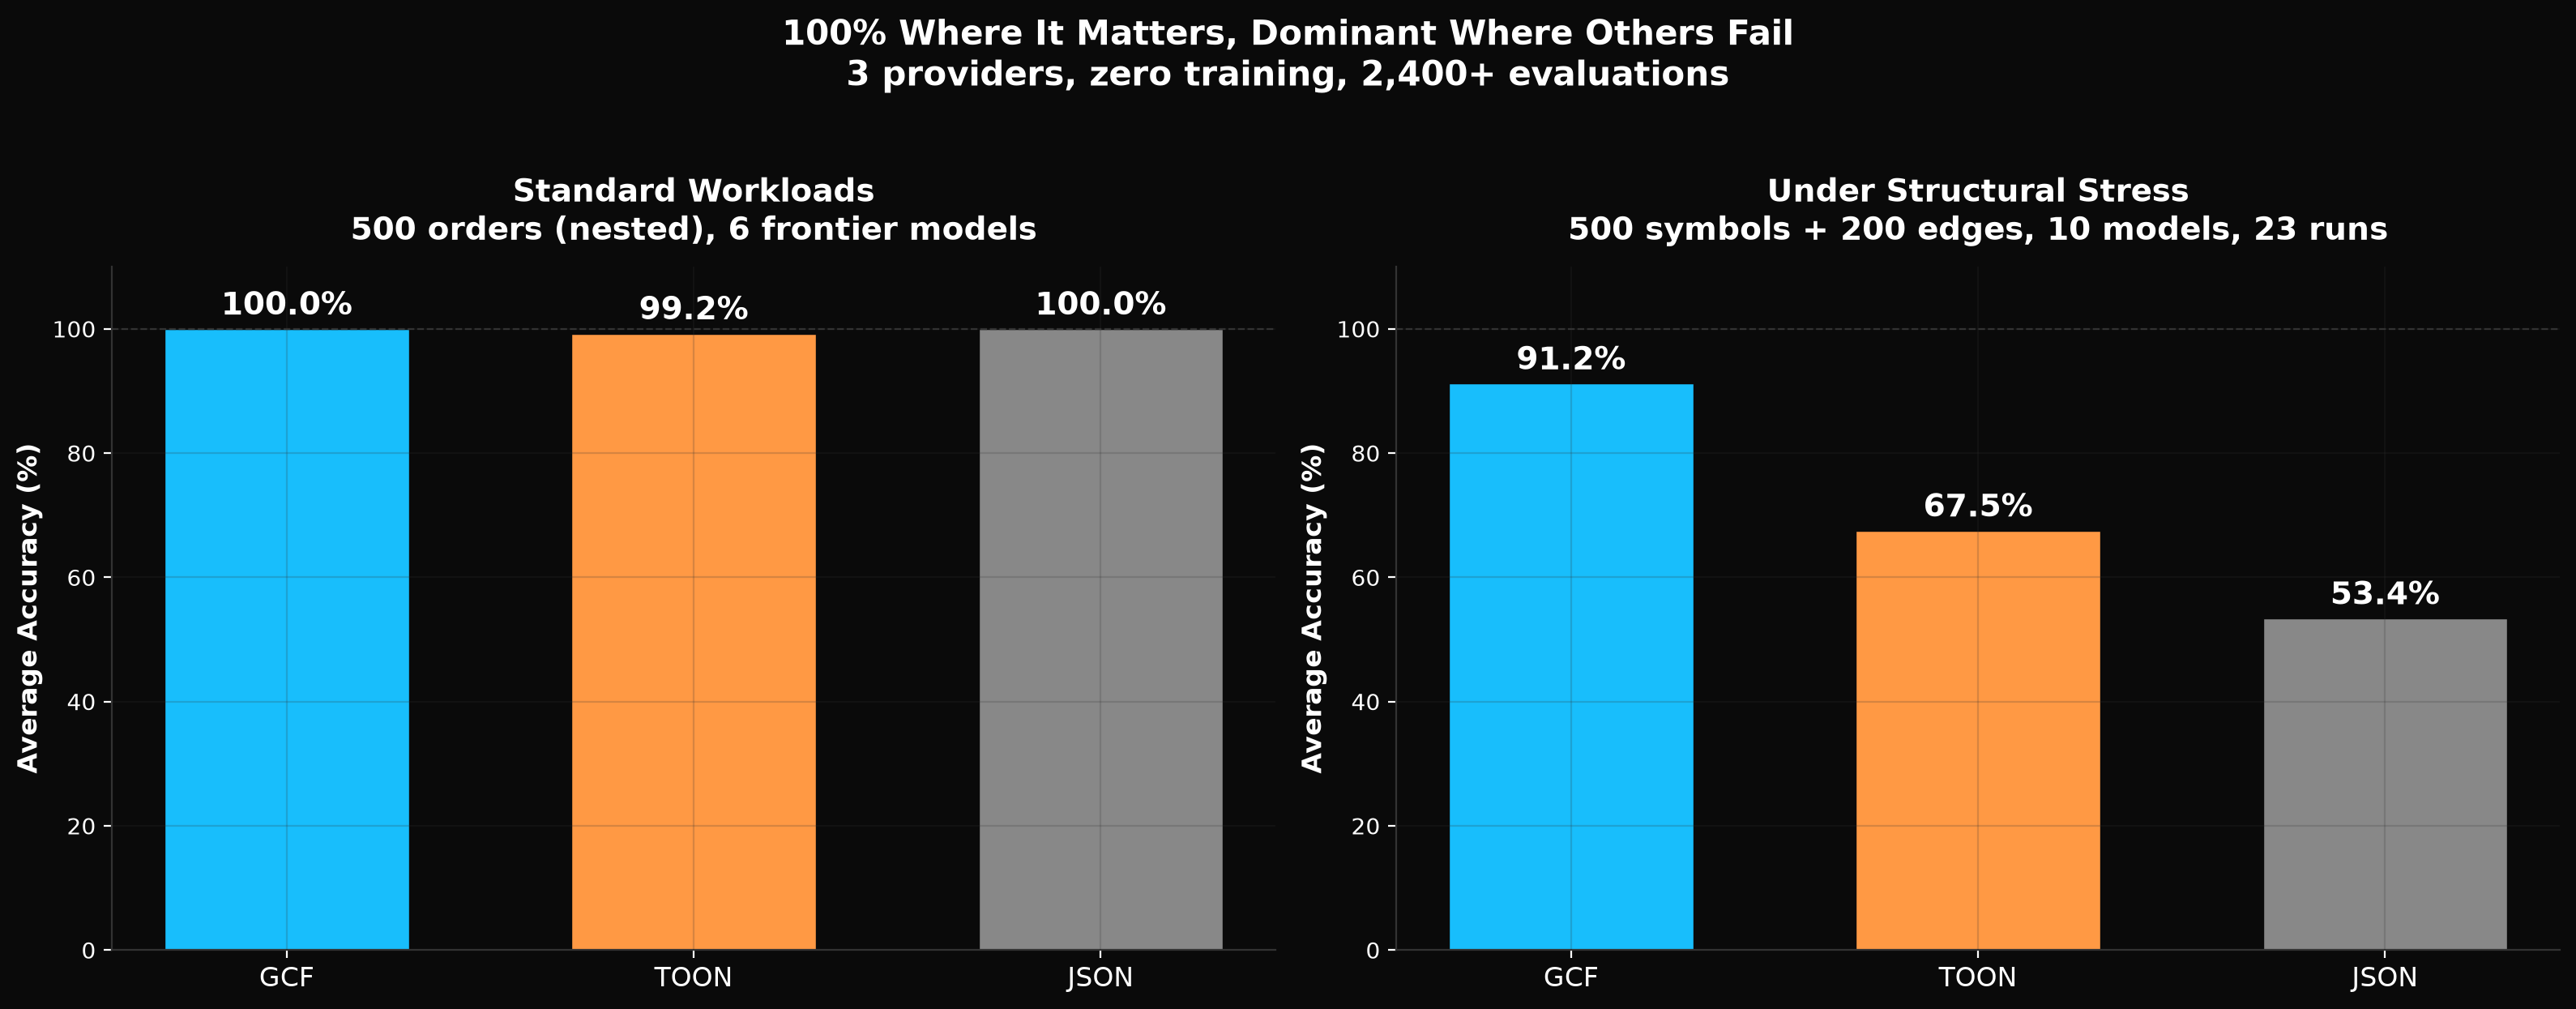
\includegraphics[keepaspectratio,alt={Comprehension and Generation across 10 models and 3 providers}]{public/charts/hero.png}}
\caption{Comprehension and Generation across 10 models and 3 providers}
\end{figure}

\begin{center}\rule{0.5\linewidth}{0.5pt}\end{center}

\subsection{1. Why JSON Fails at Scale}\label{why-json-fails-at-scale}

The Model Context Protocol (MCP) defines how AI agents interact with
external tools. Tool responses are overwhelmingly encoded as JSON. This
is convenient for developers but expensive for the consumer that matters
most: the language model itself.

Consider a typical MCP tool response returning 10 graph nodes and 8
edges (a blast radius query, a dependency subgraph, or a context
retrieval result). In JSON, this payload consumes \textasciitilde965
tokens. The same semantic content in GCF consumes \textasciitilde233
tokens. The difference, 732 tokens, is pure waste: field name
repetition, structural delimiters (\texttt{\{}, \texttt{\}},
\texttt{{[}}, \texttt{{]}}, \texttt{:}, \texttt{","}), and full
qualified names repeated in every edge reference.

This waste compounds across a task. An agent making 5 tool calls during
a code change task consumes \textasciitilde4,825 tokens on JSON tool
responses. In GCF, the same 5 calls consume \textasciitilde1,165 tokens,
and less with session statefulness enabled (previously-transmitted nodes
are referenced by local ID without retransmission). The difference,
\textasciitilde3,660 tokens, is context window capacity that could hold
source code, documentation, or additional tool results.

\subsubsection{1.1 Why This Matters Now}\label{why-this-matters-now}

Three trends make this problem urgent:

\begin{enumerate}
\def\labelenumi{\arabic{enumi}.}
\item
  \textbf{Tool-heavy agent workflows.} Modern AI agents make 10-50 tool
  calls per task. Each call returns JSON. Token budgets are consumed by
  tool overhead before the agent finishes its work.
\item
  \textbf{Graph-structured responses are growing.} Code intelligence,
  dependency analysis, knowledge graphs, and system topology queries all
  return graph data. Graph payloads are JSON's worst case because they
  contain repeated node references across edges.
\item
  \textbf{Context window costs are real.} Whether measured in dollars
  (API billing), latency (time-to-first-token), or capability (what fits
  in the window), every wasted token reduces the agent's effectiveness.
\end{enumerate}

\subsubsection{1.2 Why Not Just Use
Binary?}\label{why-not-just-use-binary}

Binary formats (Protocol Buffers, MessagePack, FlatBuffers) optimize for
byte size and decode speed. But LLMs consume text, not bytes. A
protobuf-encoded tool response must be decoded to text before the LLM
can process it, and the decoded text is typically JSON, eliminating the
savings at the point of consumption.

The optimization target is not bytes on wire. It is tokens in the
context window. These are different quantities with different solutions.

\begin{center}\rule{0.5\linewidth}{0.5pt}\end{center}

\subsection{2. Design Principles}\label{design-principles}

GCF's graph profile is designed around three observations about graph
data that JSON cannot exploit. Its generic profile (Section 3.6)
generalizes these principles to arbitrary structured data.

\subsubsection{2.1 Referential Identity}\label{referential-identity}

Graph nodes are referenced multiple times: once in their declaration and
once per edge they participate in. In JSON, each reference repeats the
full qualified name:

\begin{Shaded}
\begin{Highlighting}[]
\FunctionTok{\{}
  \DataTypeTok{"source"}\FunctionTok{:} \StringTok{"github.com/org/repo/internal/mcp.NewServer"}\FunctionTok{,}
  \DataTypeTok{"target"}\FunctionTok{:} \StringTok{"github.com/org/repo/internal/mcp.requireHash"}\FunctionTok{,}
  \DataTypeTok{"edge\_type"}\FunctionTok{:} \StringTok{"calls"}
\FunctionTok{\}}
\end{Highlighting}
\end{Shaded}

In GCF, nodes are declared once with a local ID and referenced by that
ID thereafter:

\begin{verbatim}
@0 fn github.com/org/repo/internal/mcp.requireHash 0.78 lsp_resolved
@4 fn github.com/org/repo/internal/mcp.NewServer 0.54 lsp_resolved
@0<@4 calls
\end{verbatim}

The full qualified name appears once per node. Every subsequent
reference is 2-3 tokens (\texttt{@0}, \texttt{@4}) instead of 15-20
tokens.

\subsubsection{2.2 Topological Encoding}\label{topological-encoding}

JSON encodes edges as objects with named fields. GCF encodes edges as
directed connections:

\textbf{JSON (1 edge, \textasciitilde12 tokens):}

\begin{Shaded}
\begin{Highlighting}[]
\FunctionTok{\{}\DataTypeTok{"source"}\FunctionTok{:} \StringTok{"..."}\FunctionTok{,} \DataTypeTok{"target"}\FunctionTok{:} \StringTok{"..."}\FunctionTok{,} \DataTypeTok{"edge\_type"}\FunctionTok{:} \StringTok{"calls"}\FunctionTok{\}}
\end{Highlighting}
\end{Shaded}

\textbf{GCF (1 edge, \textasciitilde5 tokens):}

\begin{verbatim}
@0<@4 calls
\end{verbatim}

The \texttt{\textless{}} arrow encodes direction. The source and target
are local IDs. The edge type is a bare token. No field names, no
delimiters, no quoting.

\subsubsection{2.3 Hierarchical Grouping}\label{hierarchical-grouping}

Graph query results often partition nodes by distance from a query
center: direct targets (distance 0), related symbols (distance 1),
extended context (distance 2+). In JSON, each node carries a
\texttt{"distance":\ N} field. In GCF, a section header replaces all
per-node distance fields:

\begin{verbatim}
## targets
@0 fn ... 0.78 lsp_resolved
@1 method ... 0.74 lsp_resolved
## related
@4 fn ... 0.54 lsp_resolved
\end{verbatim}

One header replaces N repeated fields.

\begin{center}\rule{0.5\linewidth}{0.5pt}\end{center}

\subsection{3. Specification}\label{specification}

\subsubsection{3.1 Grammar}\label{grammar}

\begin{verbatim}
payload       = header LF { section } [ summary ] ;
section       = group-header LF { line LF } ;
line          = node-line | edge-line | ref-line | tabular-row
              | kv-line | nested-ref | inline-array | comment ;
summary       = "##! summary" SP key-value { SP key-value } LF ;

header        = "GCF" SP key-value { SP key-value } ;
group-header  = "##" SP group-name [ SP "[" count-or-deferred "]" [ field-decl ] ] ;
count-or-deferred = count | "?" ;
field-decl    = "{" field-name { "," field-name } "}" ;
node-line     = "@" id SP kind SP qname SP score SP provenance ;
edge-line     = "@" target "<" "@" source SP edge-type [ SP status ] ;
ref-line      = "@" id SP SP "# previously transmitted" ;
tabular-row   = [ "@" id SP ] value { "|" value } ;
kv-line       = key "=" value ;
inline-array  = key "[" count-or-deferred "]" ":" SP value { "," value } ;
nested-ref    = "." field-name ;
comment       = "#" SP text ;

id            = DIGIT { DIGIT } ;
count         = DIGIT { DIGIT } ;
kind          = "fn" | "type" | "method" | "iface" | "var" | "const"
              | "resource" | "table" | "class" | "selector" | "field"
              | "route" | "ext" | "file" | "pkg" | "svc" ;
status        = "added" | "removed" ;
\end{verbatim}

\subsubsection{3.2 Header}\label{header}

The header line identifies the format and carries payload metadata:

\begin{verbatim}
GCF profile=graph tool=context_for_task budget=5000 tokens=1847 symbols=10 edges=8
\end{verbatim}

\texttt{tool} identifies the MCP tool that produced this response.
\texttt{budget} and \texttt{tokens} enable the consumer to assess
utilization. \texttt{symbols} and \texttt{edges} give counts without
scanning.

\subsubsection{3.3 Node Lines}\label{node-lines}

\begin{verbatim}
@{id} {kind} {qualified_name} {score} {provenance}
\end{verbatim}

Fields are positional. No field names, no delimiters beyond whitespace.
Kind abbreviations reduce token count (\texttt{fn} vs
\texttt{"function"}, \texttt{iface} vs \texttt{"interface"}).

{\def\LTcaptype{none} % do not increment counter
\begin{longtable}[]{@{}ll@{}}
\toprule\noalign{}
Abbreviation & Full form \\
\midrule\noalign{}
\endhead
\bottomrule\noalign{}
\endlastfoot
\texttt{fn} & function \\
\texttt{type} & type \\
\texttt{method} & method \\
\texttt{iface} & interface \\
\texttt{var} & var \\
\texttt{const} & const \\
\texttt{resource} & resource \\
\texttt{table} & table \\
\texttt{class} & class \\
\texttt{selector} & selector \\
\texttt{field} & field \\
\texttt{route} & route\_handler \\
\texttt{ext} & external \\
\texttt{file} & file \\
\texttt{pkg} & package \\
\texttt{svc} & service \\
\end{longtable}
}

\subsubsection{3.4 Edge Lines}\label{edge-lines}

\begin{verbatim}
@{target}<@{source} {edge_type} [{status}]
\end{verbatim}

The \texttt{\textless{}} arrow points toward the target.
\texttt{@0\textless{}@4\ calls} means ``@4 calls @0.'' Status is
optional: \texttt{added} or \texttt{removed} for diff payloads.

\subsubsection{3.5 Group Headers}\label{group-headers}

\begin{verbatim}
## targets
## related
## extended
## edges [N]
\end{verbatim}

Group headers partition the payload into semantic sections. The group a
node appears in encodes its distance from the query center, eliminating
per-node distance fields. The edges section header includes
\texttt{{[}N{]}} (the edge count) to enable direct count verification by
the LLM without scanning.

\subsubsection{3.6 Generic Profile (Generic
Encoding)}\label{generic-profile-generic-encoding}

The graph profile (Sections 3.1-3.5) encodes typed nodes and edges. The
generic profile encodes arbitrary structured data using the same grammar
primitives.

\textbf{Tabular arrays:}

\begin{verbatim}
## {name} [{count}]{{field1},{field2},{field3}}
value1|value2|value3
\end{verbatim}

The header declares field names once. Rows are pipe-separated positional
values. No field names repeated per record.

\begin{verbatim}
## employees [3]{id,name,department,salary}
1|Alice Smith|Engineering|95000
2|Bob Jones|Sales|72000
3|Carol Wu|Marketing|85000
\end{verbatim}

\textbf{Primitive arrays} (all elements are scalars) are inlined on a
single line:

\begin{verbatim}
tags[3]: production,us-east-1,critical
ports[3]: 8080,8443,9090
\end{verbatim}

\textbf{Key-value pairs} for primitive object fields:

\begin{verbatim}
config=production
port=5432
active=true
\end{verbatim}

\textbf{Section headers} for nested objects:

\begin{verbatim}
## database
  host=db.example.com
  port=5432
\end{verbatim}

\textbf{Nested fields in tabular rows} use \texttt{@\{id\}} prefixes and
\texttt{.field\ \{\}}:

\begin{verbatim}
## orders [2]{id,total,status,customer}
@0 1001|249.99|shipped|^
  .customer {}
    name=Alice Smith
    tier=premium
\end{verbatim}

\textbf{Value encoding rules:}

{\def\LTcaptype{none} % do not increment counter
\begin{longtable}[]{@{}ll@{}}
\toprule\noalign{}
Type & Encoding \\
\midrule\noalign{}
\endhead
\bottomrule\noalign{}
\endlastfoot
String & bare text \\
Number & unquoted decimal \\
Boolean & lowercase \texttt{true}/\texttt{false} \\
Null & \texttt{-} \\
Empty string & \texttt{""} \\
String containing \texttt{\textbar{}} or \texttt{\textbackslash{}n} &
quoted, with \texttt{\textbackslash{}"} and
\texttt{\textbackslash{}\textbackslash{}} escaping \\
\end{longtable}
}

\textbf{Uniformity detection:} An array is tabular-eligible if the first
5 elements are objects with at least 70\% key overlap with the first
element, accommodating semi-uniform data.

\subsubsection{3.7 Session Statefulness}\label{session-statefulness}

Across multiple tool calls in a session, previously-transmitted nodes
can be referenced without retransmission:

\begin{verbatim}
GCF profile=graph tool=context_for_files tokens=800 symbols=5 edges=1 session=true
## targets
@0  # previously transmitted
@7 fn github.com/org/repo/internal/mcp.handleBlastRadius 0.62 lsp_resolved
## edges [1]
@0<@7 calls
\end{verbatim}

The \texttt{session=true} header flag enables ID persistence. A bare
\texttt{@0} (no kind, name, or score) references a node transmitted in a
previous response. Multi-call workflows get progressively cheaper as the
session builds a shared vocabulary.

This exploits a property unique to agent tool interactions: the consumer
(the LLM) maintains conversational state across calls. A traditional
wire format cannot assume its consumer remembers previous messages. GCF
can because LLM context windows are, by definition, stateful.

\subsubsection{3.8 Streaming Encoding
Extension}\label{streaming-encoding-extension}

When the encoder does not know payload size upfront (data arriving
incrementally from a database cursor, API pagination, or graph
traversal), it uses streaming mode:

\begin{verbatim}
GCF profile=graph tool=context_for_task budget=5000
## targets
@0 fn pkg.Auth 0.95 lsp_resolved
@1 fn pkg.Handler 0.88 lsp_resolved
## related
@2 type pkg.Config 0.72 ast_inferred
## edges [?]
@0<@1 calls
@2<@0 references
##! summary counts=2
\end{verbatim}

The \texttt{{[}?{]}} deferred count marker signals that the count will
be provided in the trailer. The \texttt{\#\#!\ summary} line provides
all counts after the data is complete. The LLM has both the data and the
counts in its context window (recency bias in transformer attention
means the trailer is at least as strong a signal as header counts).

Streaming mode enables zero-buffering encode: rows emit the instant they
are produced, with O(1) memory per row. This is critical for MCP servers
that walk large graphs or paginate results; the LLM starts receiving
context immediately instead of waiting for the full traversal.

TOON cannot add streaming without a breaking spec change (their grammar
mandates upfront \texttt{{[}N{]}} with no deferred count or trailer
mechanism).

\begin{center}\rule{0.5\linewidth}{0.5pt}\end{center}

\subsection{4. Implementation Status}\label{implementation-status}

GCF is not a speculative format proposal. It is implemented in six
languages, all at v1.0.0+, published to seven package registries,
covered by 141 conformance fixtures, verified across 200M+
property-based round-trips and 7.9M fuzz executions, and deployed in
production MCP servers.

The implementation includes:

\begin{itemize}
\tightlist
\item
  \textbf{Go library} (\texttt{github.com/blackwell-systems/gcf-go},
  v1.0.2): Encode, Decode, EncodeGeneric, DecodeGeneric,
  EncodeWithSession, EncodeDelta, StreamEncoder, GenericStreamEncoder,
  ParseJSONOrdered, PackRoot. CLI with both profiles. Zero dependencies.
\item
  \textbf{TypeScript library} (\texttt{@blackwell-systems/gcf} on npm,
  v1.0.1): encode, decode, encodeGeneric, decodeGeneric,
  encodeWithSession, encodeDelta, StreamEncoder, GenericStreamEncoder.
  CLI with both profiles. Zero dependencies, ESM.
\item
  \textbf{Python library} (\texttt{gcf-python} on PyPI, v1.0.1): encode,
  decode, encode\_generic, decode\_generic, encode\_with\_session,
  encode\_delta, StreamEncoder, GenericStreamEncoder. CLI with both
  profiles. Zero dependencies, Python 3.9+.
\item
  \textbf{Rust library} (\texttt{gcf} on crates.io, v1.0.1): encode,
  decode, encode\_generic, decode\_generic, encode\_with\_session,
  encode\_delta, StreamEncoder, GenericStreamEncoder. CLI with both
  profiles. Minimal dependencies (serde\_json).
\item
  \textbf{Swift library} (\texttt{gcf-swift} via SPM, v1.0.1): encode,
  decode, encodeGeneric, decodeGeneric, encodeWithSession, encodeDelta,
  StreamEncoder, GenericStreamEncoder, OrderedDictionary. CLI with both
  profiles. 50M property-based round-trips. Zero dependencies.
\item
  \textbf{Kotlin library} (\texttt{gcf-kotlin} via JitPack, v1.0.1):
  encode, decode, encodeGeneric, decodeGeneric, encodeWithSession,
  encodeDelta, StreamEncoder, GenericStreamEncoder. CLI with both
  profiles. Zero dependencies.
\item
  \textbf{MCP proxy} (\texttt{github.com/blackwell-systems/gcf-proxy},
  v0.10.0): bidirectional translation (JSON-to-GCF responses,
  GCF-to-JSON requests), session dedup (40\% savings proven e2e),
  proxy-level delta encoding (68\% savings on incremental changes), HTTP
  backend (\texttt{-\/-upstream}), HTTP/SSE frontend
  (\texttt{-\/-http}), response caching (\texttt{-\/-cache}), min-size
  bypass (default 100 bytes), streaming progress notifications. Zero
  code changes to upstream.
\item
  \textbf{Cross-language matrix}: 5x5 encode/decode matrix verified (all
  passing). Each language's encoder output decoded by every other
  language's decoder.
\item
  \textbf{Conformance test suite} (141 v2 fixtures across both
  profiles): language-agnostic JSON fixtures validating encode, decode,
  session, delta, generic, streaming, and normative error cases.
\item
  \textbf{Specification} (gcformat.com, v2.0 Stable): RFC 2119 keywords,
  conformance checklists, decoder error taxonomy, streaming extension,
  security considerations, i18n, status lifecycle.
\end{itemize}

\subsubsection{Correctness Validation}\label{correctness-validation}

All six implementations are tested against round-trip invariants and the
shared conformance suite. A graph response encoded as GCF and decoded
back must preserve node identity, kind, score, provenance, group
membership, edge direction, edge type, and optional status metadata. The
generic profile is validated against additional fixtures covering flat
arrays, nested objects, value formatting, primitive array inlining, and
edge cases.

\begin{itemize}
\tightlist
\item
  \textbf{200M+ property-based round-trips} across all languages (random
  + adversarial value generators)
\item
  \textbf{7.9M fuzz executions} (Go native fuzzing) finding and fixing 3
  bugs
\item
  \textbf{141 conformance fixtures} across both profiles, streaming, and
  normative error cases
\item
  \textbf{5x5 cross-language encode/decode matrix} verified (each
  encoder's output decoded by every other decoder)
\item
  \textbf{JSON Schema validation} works on decoded output unchanged
  (gcformat.com/guide/schema-validation)
\end{itemize}

\subsubsection{Production Deployment}\label{production-deployment}

\begin{itemize}
\tightlist
\item
  \textbf{knowing} (28 MCP tools): GCF as primary output format for code
  intelligence, with session deduplication and delta encoding.
\item
  \textbf{agent-lsp} (66 MCP tools): GCF graph profile output for
  symbol-returning tools (blast\_radius, find\_callers, explore\_symbol,
  find\_references, type\_hierarchy, list\_symbols, find\_symbol,
  cross\_repo). First independent production consumer.
\item
  \textbf{NeuroNest} (NETGVai): first independent commercial adoption.
  GCF encoder in tool executor, swarm coordinator, and MCP server
  manager.
\item
  \textbf{gcf-proxy session dedup} proven end-to-end: 40\% savings on
  repeated queries, compounding across a session. Tested against
  agent-lsp on real TypeScript codebase.
\end{itemize}

\begin{center}\rule{0.5\linewidth}{0.5pt}\end{center}

\subsection{5. Where Token Savings Come
From}\label{where-token-savings-come-from}

The savings decompose into five sources:

{\def\LTcaptype{none} % do not increment counter
\begin{longtable}[]{@{}
  >{\raggedright\arraybackslash}p{(\linewidth - 6\tabcolsep) * \real{0.1569}}
  >{\raggedright\arraybackslash}p{(\linewidth - 6\tabcolsep) * \real{0.2157}}
  >{\raggedright\arraybackslash}p{(\linewidth - 6\tabcolsep) * \real{0.1961}}
  >{\raggedright\arraybackslash}p{(\linewidth - 6\tabcolsep) * \real{0.4314}}@{}}
\toprule\noalign{}
\begin{minipage}[b]{\linewidth}\raggedright
Source
\end{minipage} & \begin{minipage}[b]{\linewidth}\raggedright
JSON cost
\end{minipage} & \begin{minipage}[b]{\linewidth}\raggedright
GCF cost
\end{minipage} & \begin{minipage}[b]{\linewidth}\raggedright
Savings per occurrence
\end{minipage} \\
\midrule\noalign{}
\endhead
\bottomrule\noalign{}
\endlastfoot
Field names & 9 field names x \textasciitilde2 tokens each =
\textasciitilde18 tokens/symbol & 0 (positional) & \textasciitilde18
tokens/symbol \\
Edge references & 2 qualified names x \textasciitilde15 tokens =
\textasciitilde30 tokens/edge & 2 local IDs x \textasciitilde1 token =
\textasciitilde2 tokens/edge & \textasciitilde28 tokens/edge \\
Structural delimiters & \texttt{\{}, \texttt{\}}, \texttt{{[}},
\texttt{{]}}, \texttt{:}, \texttt{","} = \textasciitilde6 tokens/symbol
& 0 & \textasciitilde6 tokens/symbol \\
Distance fields & \texttt{"distance":\ N} = \textasciitilde3
tokens/symbol & 0 (implicit in group) & \textasciitilde3
tokens/symbol \\
Kind strings & \texttt{"function"} = \textasciitilde2 tokens &
\texttt{fn} = 1 token & \textasciitilde1 token/symbol \\
\end{longtable}
}

For a 10-symbol, 8-edge payload: JSON \textasciitilde965 tokens, GCF
\textasciitilde233 tokens. The 732-token difference breaks down roughly
as: 280 from field name elimination, 224 from edge reference
compression, 60 from delimiter removal, 30 from group headers, and the
remainder from kind abbreviations and whitespace.

\subsubsection{5.1 Generic Profile
Savings}\label{generic-profile-savings}

The generic profile achieves savings through a subset of the same
mechanisms:

{\def\LTcaptype{none} % do not increment counter
\begin{longtable}[]{@{}
  >{\raggedright\arraybackslash}p{(\linewidth - 6\tabcolsep) * \real{0.1569}}
  >{\raggedright\arraybackslash}p{(\linewidth - 6\tabcolsep) * \real{0.2157}}
  >{\raggedright\arraybackslash}p{(\linewidth - 6\tabcolsep) * \real{0.1961}}
  >{\raggedright\arraybackslash}p{(\linewidth - 6\tabcolsep) * \real{0.4314}}@{}}
\toprule\noalign{}
\begin{minipage}[b]{\linewidth}\raggedright
Source
\end{minipage} & \begin{minipage}[b]{\linewidth}\raggedright
JSON cost
\end{minipage} & \begin{minipage}[b]{\linewidth}\raggedright
GCF cost
\end{minipage} & \begin{minipage}[b]{\linewidth}\raggedright
Savings per occurrence
\end{minipage} \\
\midrule\noalign{}
\endhead
\bottomrule\noalign{}
\endlastfoot
Field names & repeated per record & declared once in header &
\textasciitilde(N-1) x fields per array \\
Structural delimiters & \texttt{\{}, \texttt{\}}, \texttt{:},
\texttt{,}, \texttt{"} per record & \texttt{\textbar{}} between values &
\textasciitilde6 tokens/record \\
Array framing & \texttt{{[}}, \texttt{{]}}, commas &
\texttt{{[}count{]}} in header & fixed \\
Primitive arrays & \texttt{{[}"a","b","c"{]}} with brackets and quotes &
\texttt{name{[}3{]}:\ a,b,c} & \textasciitilde50\% per array \\
Nesting & braces + field names & \texttt{.field\ \{\}} +
\texttt{key=value} & \textasciitilde50\% per nested object \\
\end{longtable}
}

For 2,000 employee records with 6 fields: JSON \textasciitilde127,050
tokens, GCF \textasciitilde49,055 tokens (61\% savings). On TOON's
benchmark, GCF's generic profile uses 34\% fewer tokens than TOON on
mixed-structure data and wins all 6 datasets.

\begin{center}\rule{0.5\linewidth}{0.5pt}\end{center}

\subsection{6. Benchmarks}\label{benchmarks}

All benchmarks encode the same semantic content in JSON and GCF. Token
counts in Section 6.1 use cl100k\_base; the 500-symbol eval (Section
6.1a) and TOON comparison (Section 8.5) use o200k\_base (matching TOON's
benchmark methodology). Measurements taken on Apple M4 Pro.

\subsubsection{6.1 Token Comparison}\label{token-comparison}

{\def\LTcaptype{none} % do not increment counter
\begin{longtable}[]{@{}llllll@{}}
\toprule\noalign{}
Payload & Symbols & Edges & JSON tokens & GCF tokens & Savings \\
\midrule\noalign{}
\endhead
\bottomrule\noalign{}
\endlastfoot
context\_for\_task & 10 & 8 & 965 & 233 & 75.9\% \\
context\_for\_task (large) & 30 & 24 & 2,968 & 649 & 78.1\% \\
context\_for\_files & 15 & 12 & 1,490 & 334 & 77.6\% \\
blast\_radius & 8 & 6 & 835 & 208 & 75.1\% \\
semantic\_diff & 12 & 10 & 1,206 & 295 & 75.5\% \\
graph\_query & 20 & 16 & 2,078 & 423 & 79.6\% \\
\end{longtable}
}

\textbf{Median token savings: 76.7\%}

Savings increase with payload size because the ratio of edge references
to node declarations grows, and edge references are where compression is
strongest.

\subsubsection{6.1a Comprehension Accuracy at Scale (500 symbols,
multi-model)}\label{a-comprehension-accuracy-at-scale-500-symbols-multi-model}

23 comprehension runs across 10 models and 3 providers. 500 symbols, 200
edges, 13 structured extraction questions with deterministic ground
truth (no LLM judge). Each run generates a fresh random payload. Zero
format instructions in the prompt.

{\def\LTcaptype{none} % do not increment counter
\begin{longtable}[]{@{}lllll@{}}
\toprule\noalign{}
Model & Runs & GCF avg & TOON avg & JSON avg \\
\midrule\noalign{}
\endhead
\bottomrule\noalign{}
\endlastfoot
Claude Opus 4.6 & 2 & \textbf{96.2\%} & 84.6\% & 73.1\% \\
Claude Sonnet 4.6 & 2 & \textbf{100\%} & 73.1\% & 53.8\% \\
Claude Haiku 4.5 & 2 & \textbf{96.2\%} & 69.2\% & 57.7\% \\
GPT-5.5 & 5 & \textbf{84.1\%} & 67.7\% & 45.8\% \\
GPT-5.4 & 4 & \textbf{78.0\%} & 56.0\% & 44.1\% \\
GPT-5.4-mini & 2 & \textbf{71.8\%} & 64.1\% & 54.2\% \\
Gemini 2.5 Pro & 1 & \textbf{100\%} & 76.9\% & 58.3\% \\
Gemini 3.1 Pro & 1 & \textbf{100\%} & 76.9\% & 46.2\% \\
Gemini 3.5 Flash & 1 & \textbf{100\%} & 61.5\% & 46.2\% \\
Gemini 2.5 Flash & 3 & \textbf{80.6\%} & 54.6\% & 57.0\% \\
\end{longtable}
}

\textbf{GCF wins 22 of 23 runs (1 tie, 0 losses).} Four models achieve
100\%.

\begin{figure}
\centering
\pandocbounded{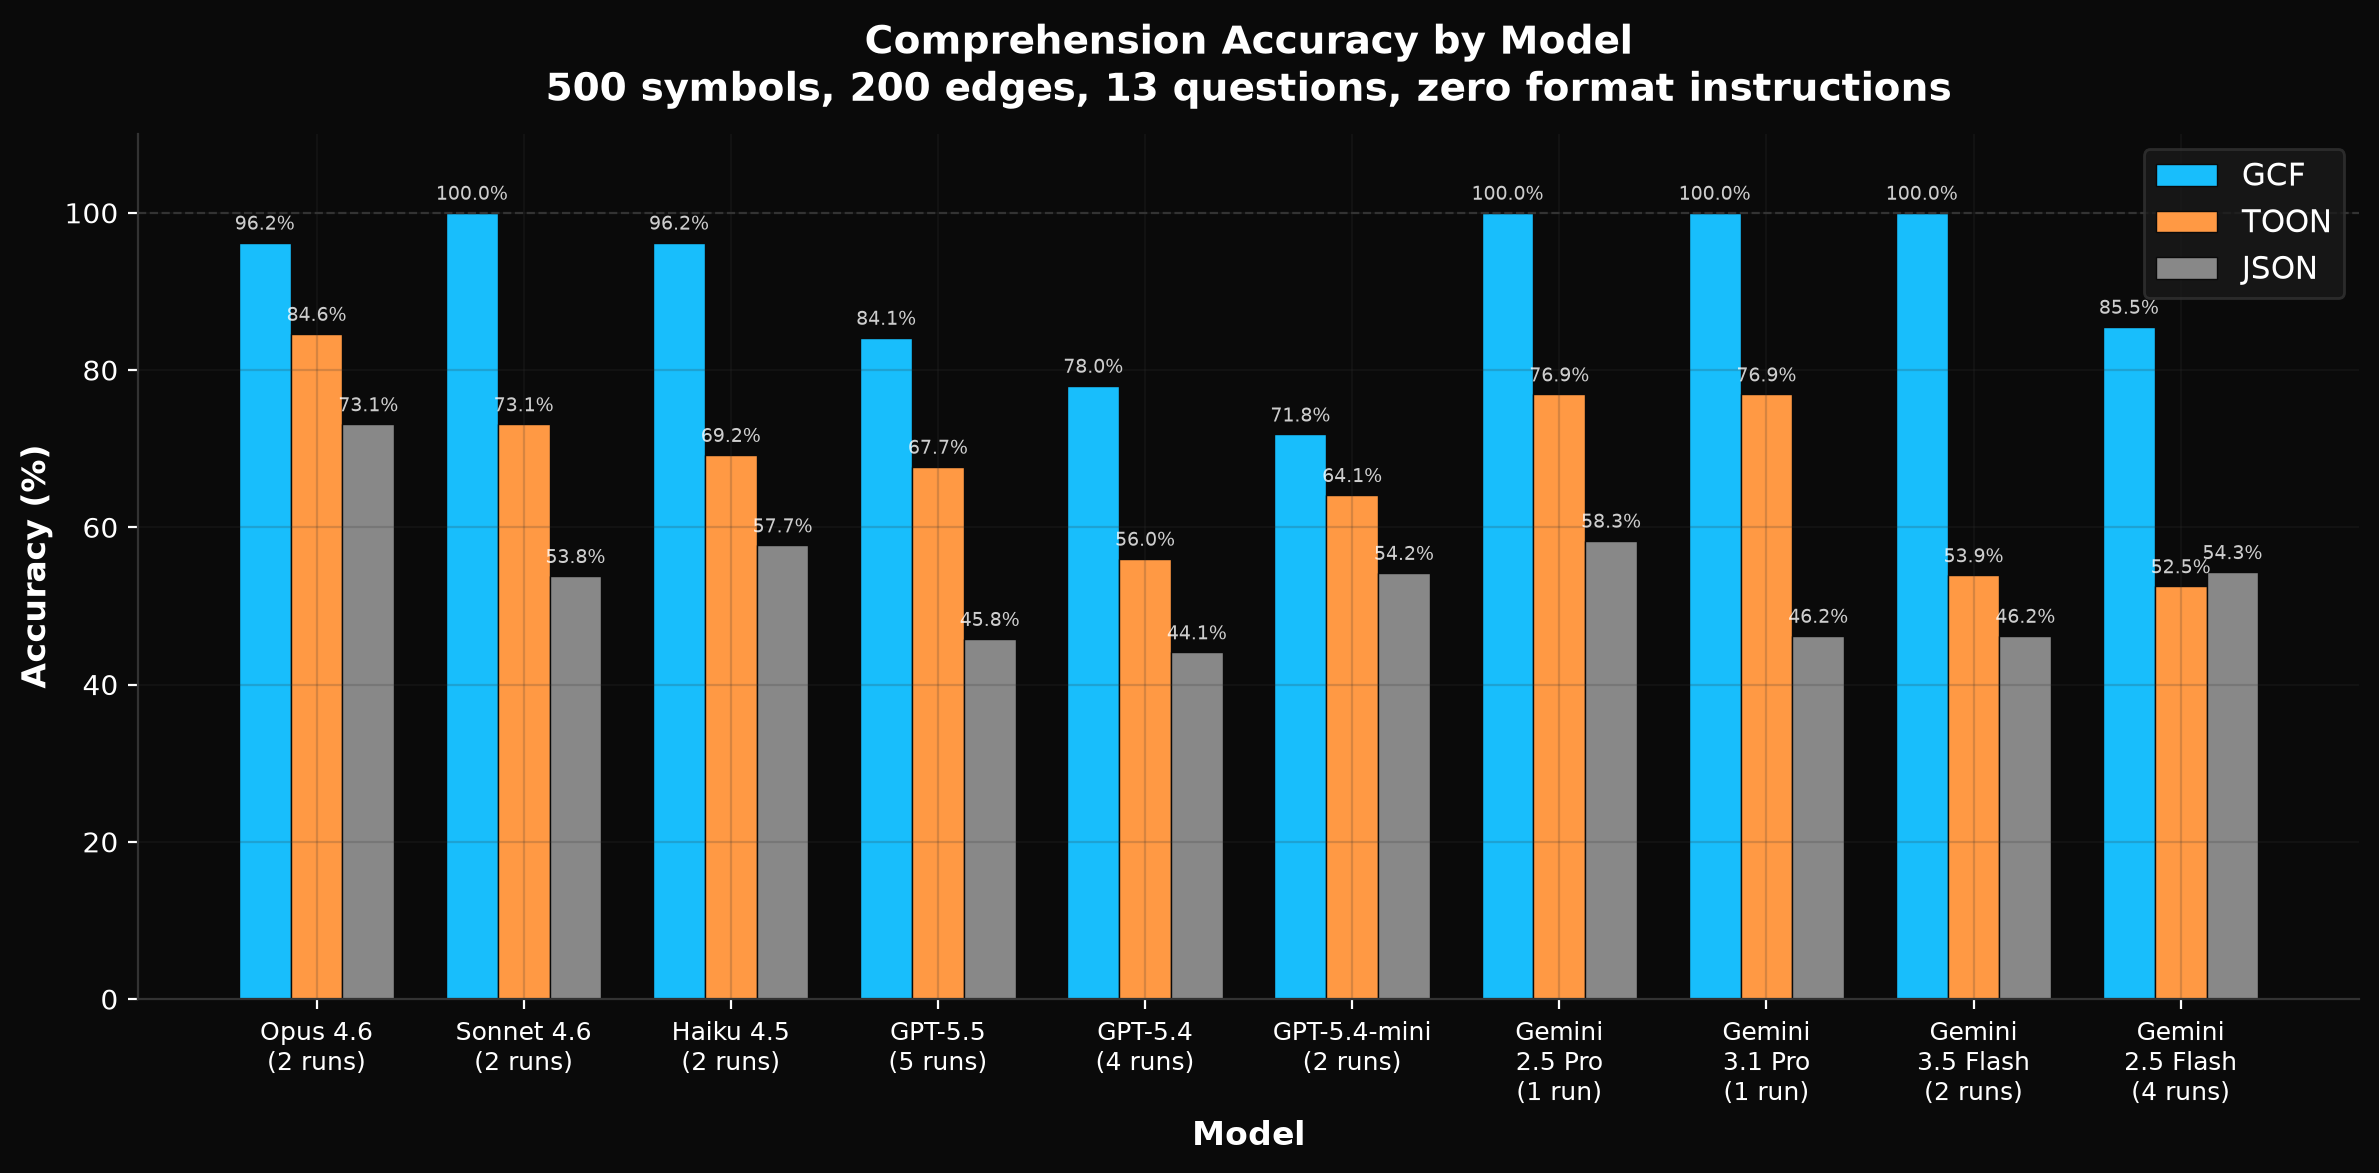
\includegraphics[keepaspectratio,alt={Comprehension Accuracy by Model}]{public/charts/accuracy-by-model.png}}
\caption{Comprehension Accuracy by Model}
\end{figure}

\begin{figure}
\centering
\pandocbounded{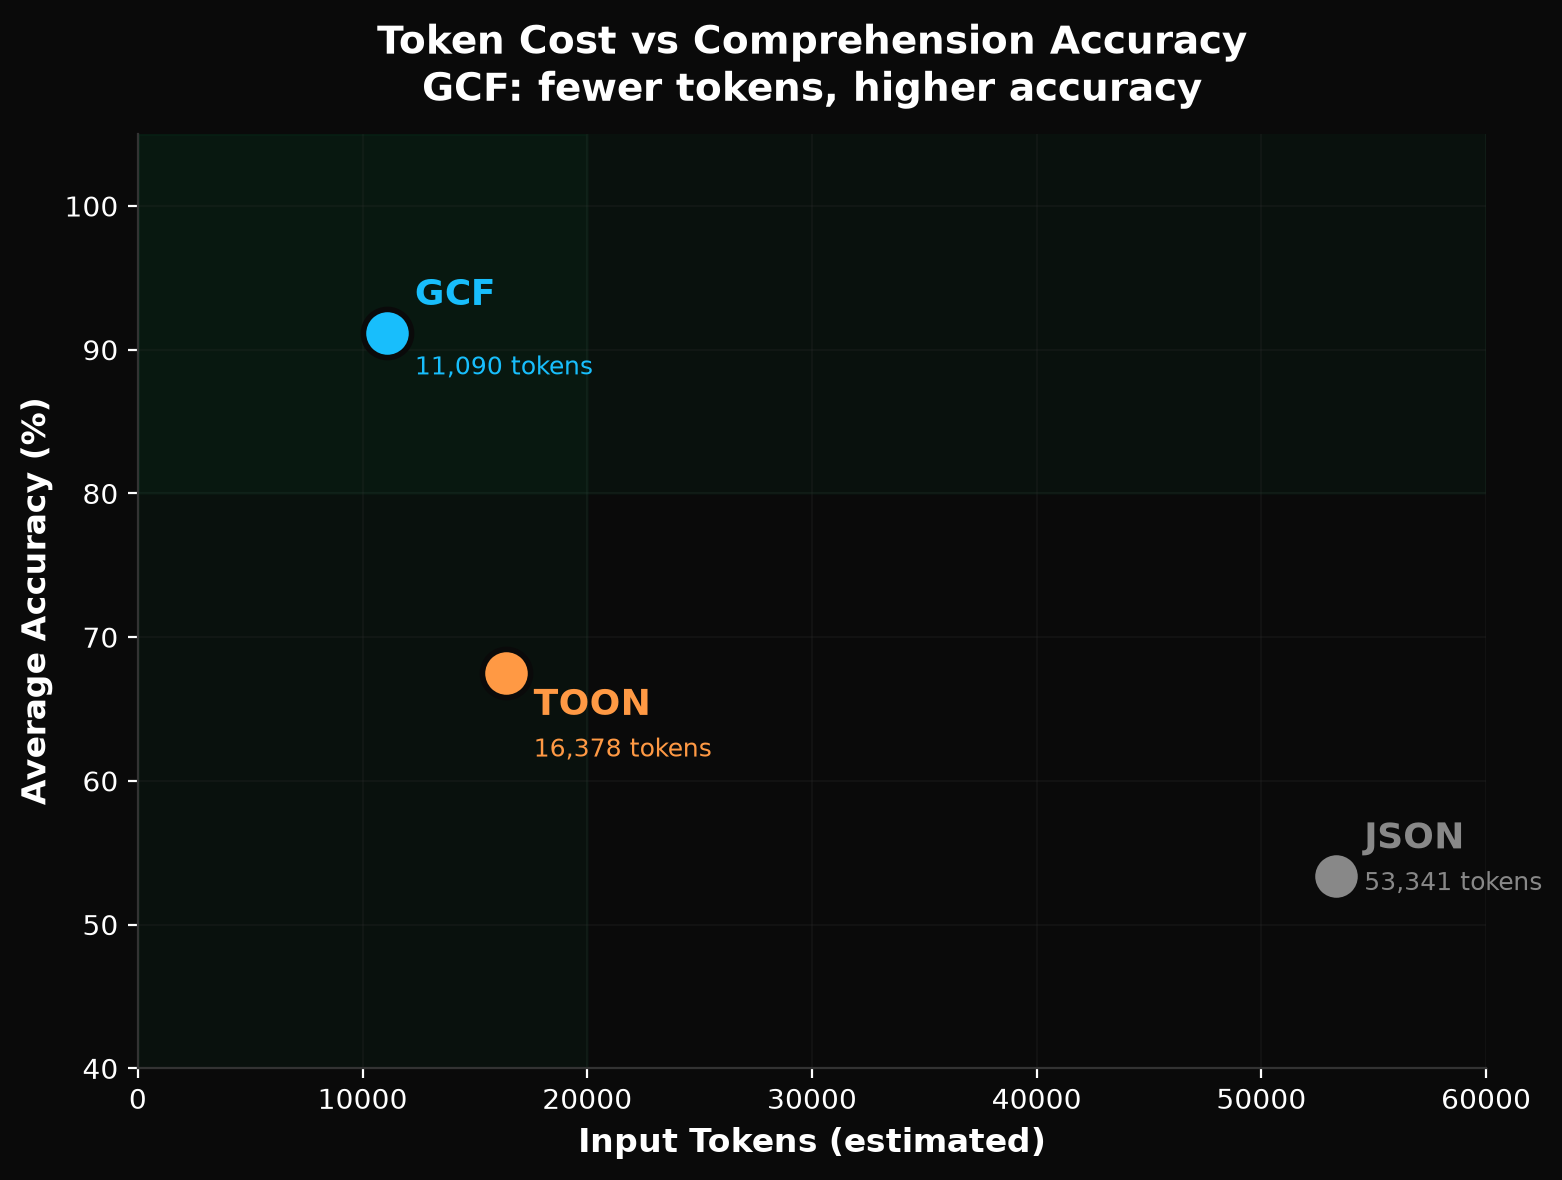
\includegraphics[keepaspectratio,alt={Token Cost vs Comprehension Accuracy}]{public/charts/tokens-vs-accuracy.png}}
\caption{Token Cost vs Comprehension Accuracy}
\end{figure}

\paragraph{Failure taxonomy}\label{failure-taxonomy}

GCF, TOON, and JSON produce qualitatively different failure modes:

\textbf{GCF fails on precision} (median error: 4). Off-by-1 header
misreads (5 occurrences), deterministic column scan miscounts on GPT-5.4
(10), and context overwhelm empty responses on GPT-5.5 (10). The format
structure is understood; the count is slightly misread.

\textbf{TOON fails on comprehension} (median error: 53). Distance
grouping failures across all models (25 occurrences), round-number
guessing where the model gives up counting (7), attention decay on the
last row (5), and context overwhelm (20). The model cannot filter a flat
500-row table by column value.

\textbf{JSON fails on structural overwhelm} (median error: 56). Empty
string responses where the model produces nothing (33), massive
undercounts (9), distance filter failures (29), and field confusion (3).
At 53,000 tokens of repeated field names, the format itself prevents
comprehension.

On two separate runs, Claude Opus responded to a JSON counting question
by manually enumerating symbols one by one (143 lines on run 1, 119 on
run 2), burning output tokens on a chain-of-thought enumeration and
still getting the wrong answer. GCF answers the same question from a
3-character header: \texttt{{[}167{]}}.

\begin{figure}
\centering
\pandocbounded{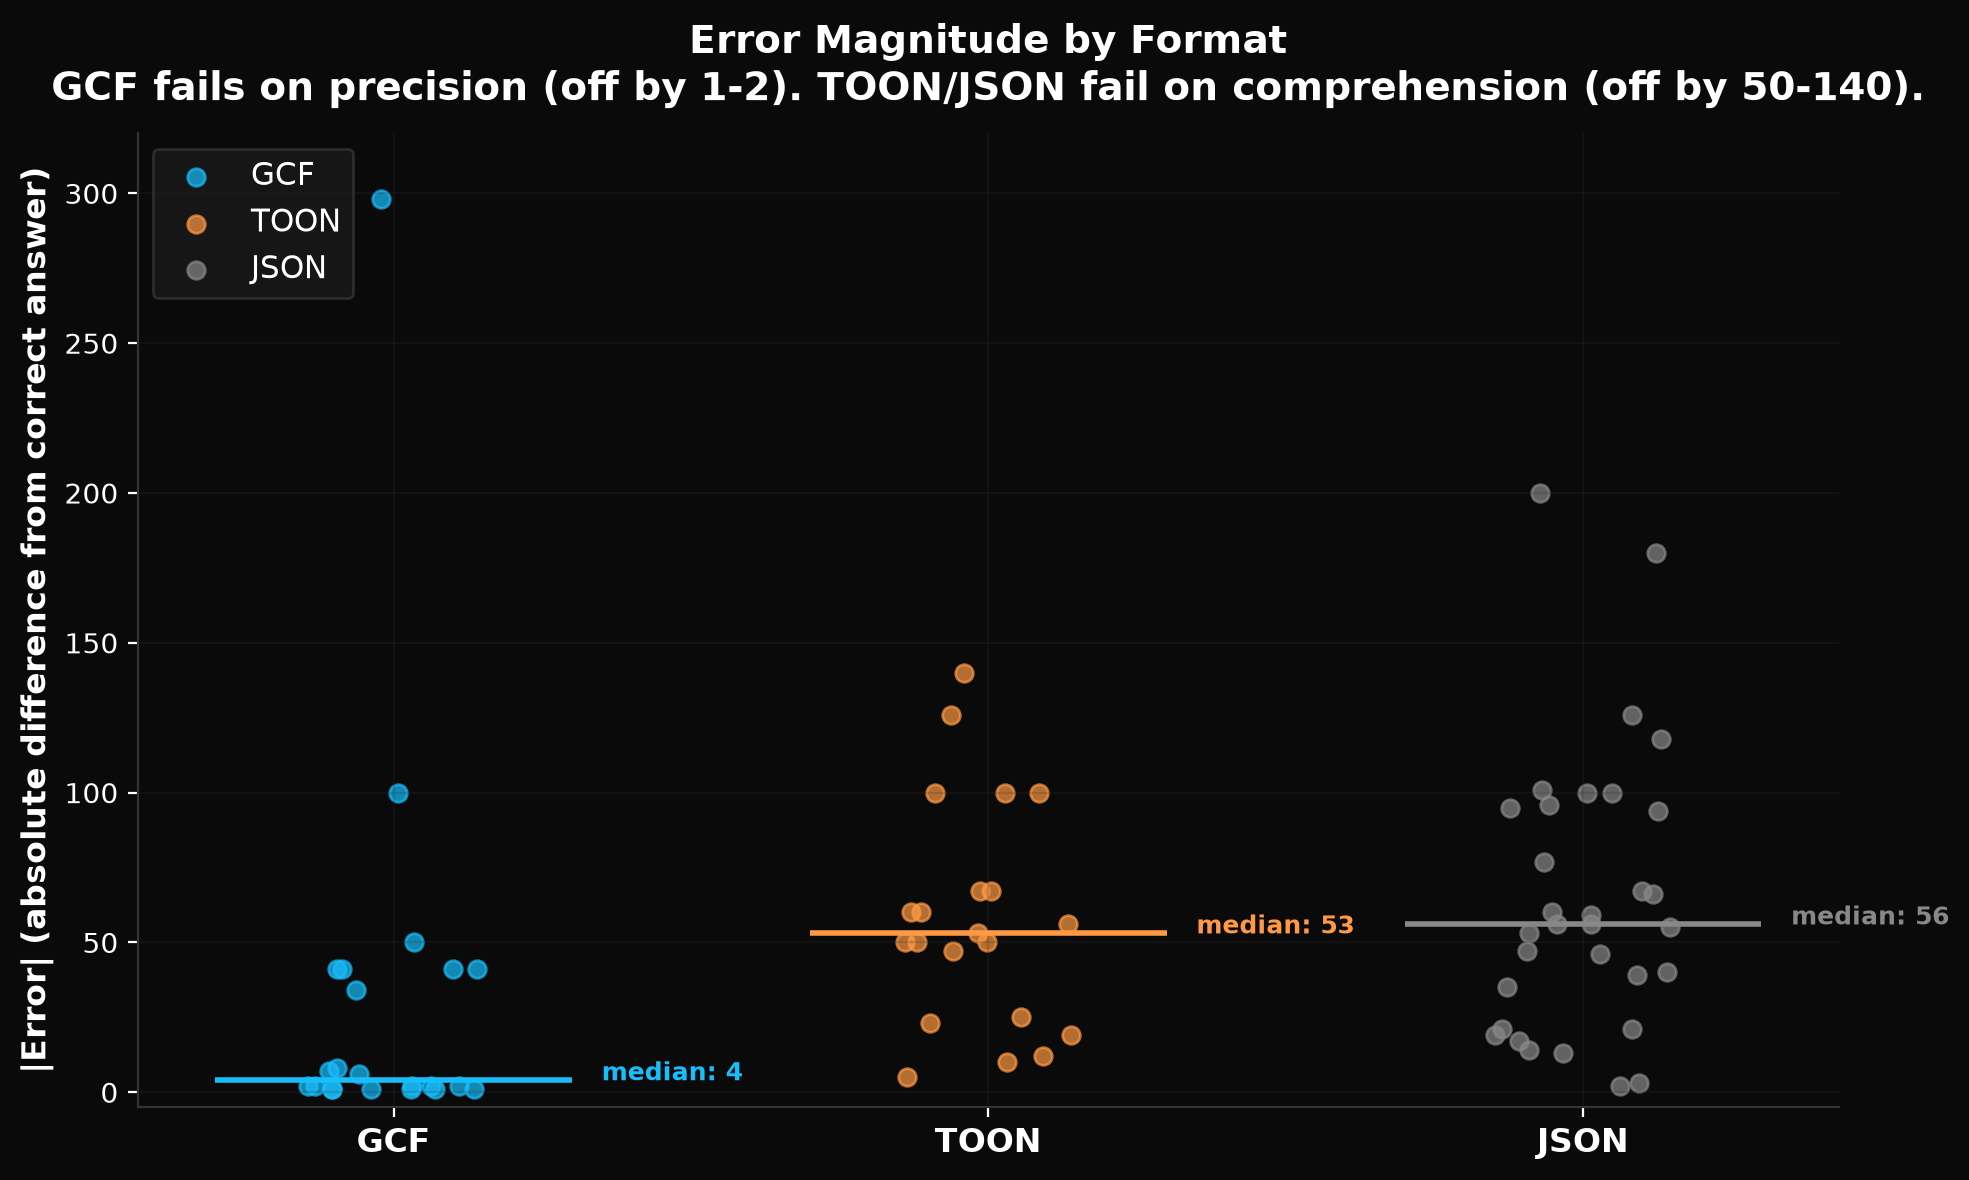
\includegraphics[keepaspectratio,alt={Error Magnitude by Format}]{public/charts/error-magnitude.png}}
\caption{Error Magnitude by Format}
\end{figure}

\begin{figure}
\centering
\pandocbounded{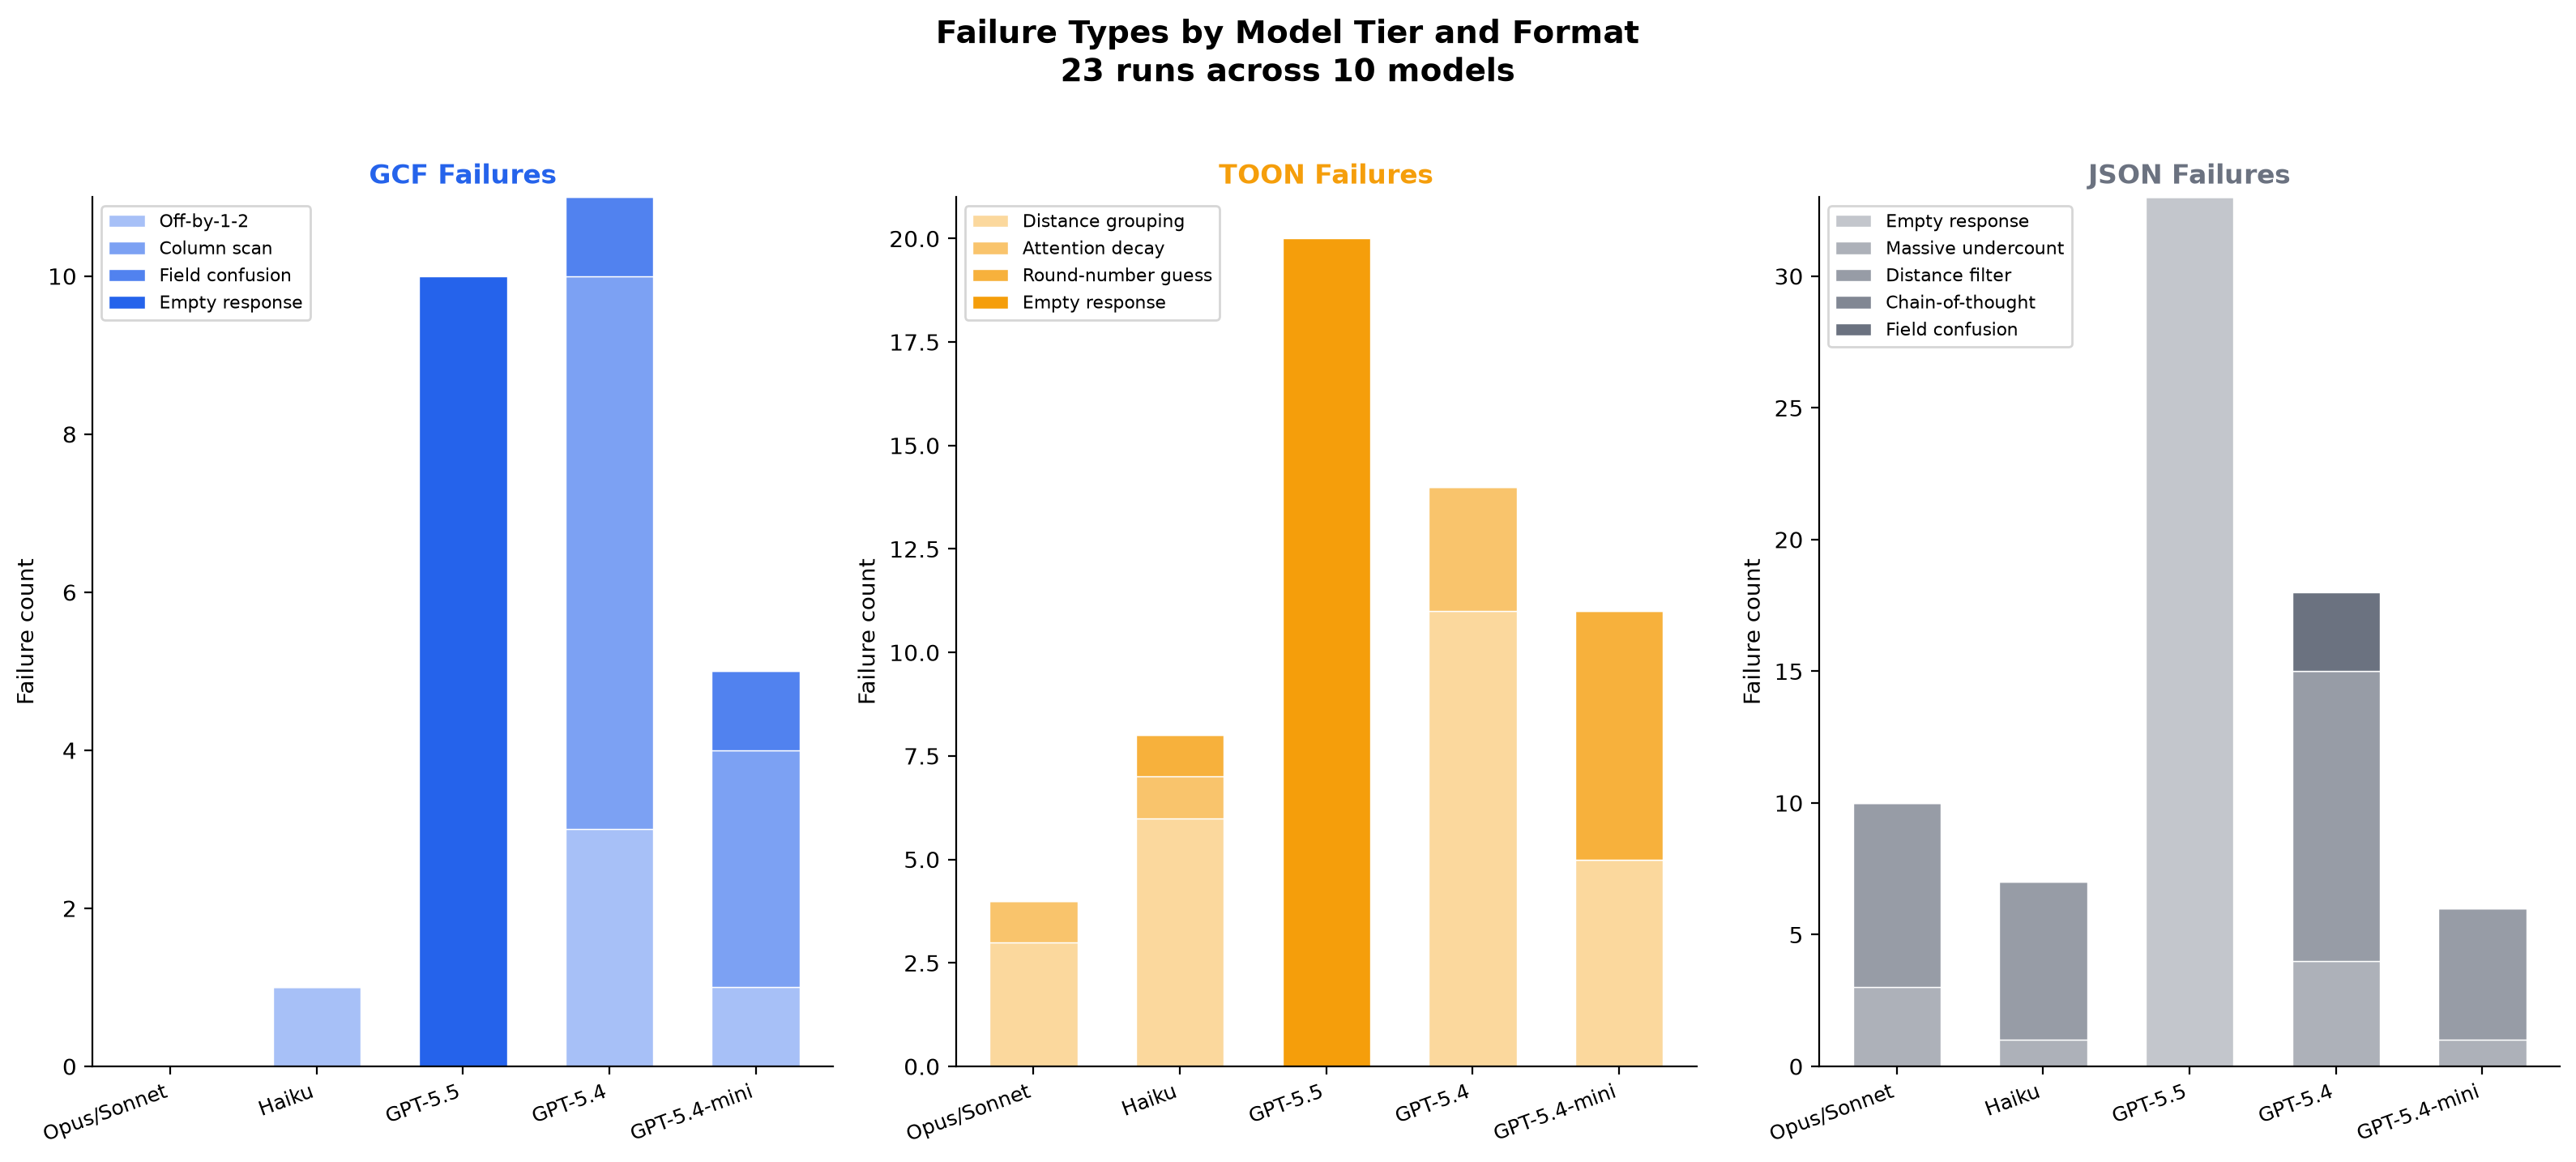
\includegraphics[keepaspectratio,alt={Failure Types by Model Tier}]{public/charts/failure-types.png}}
\caption{Failure Types by Model Tier}
\end{figure}

\begin{figure}
\centering
\pandocbounded{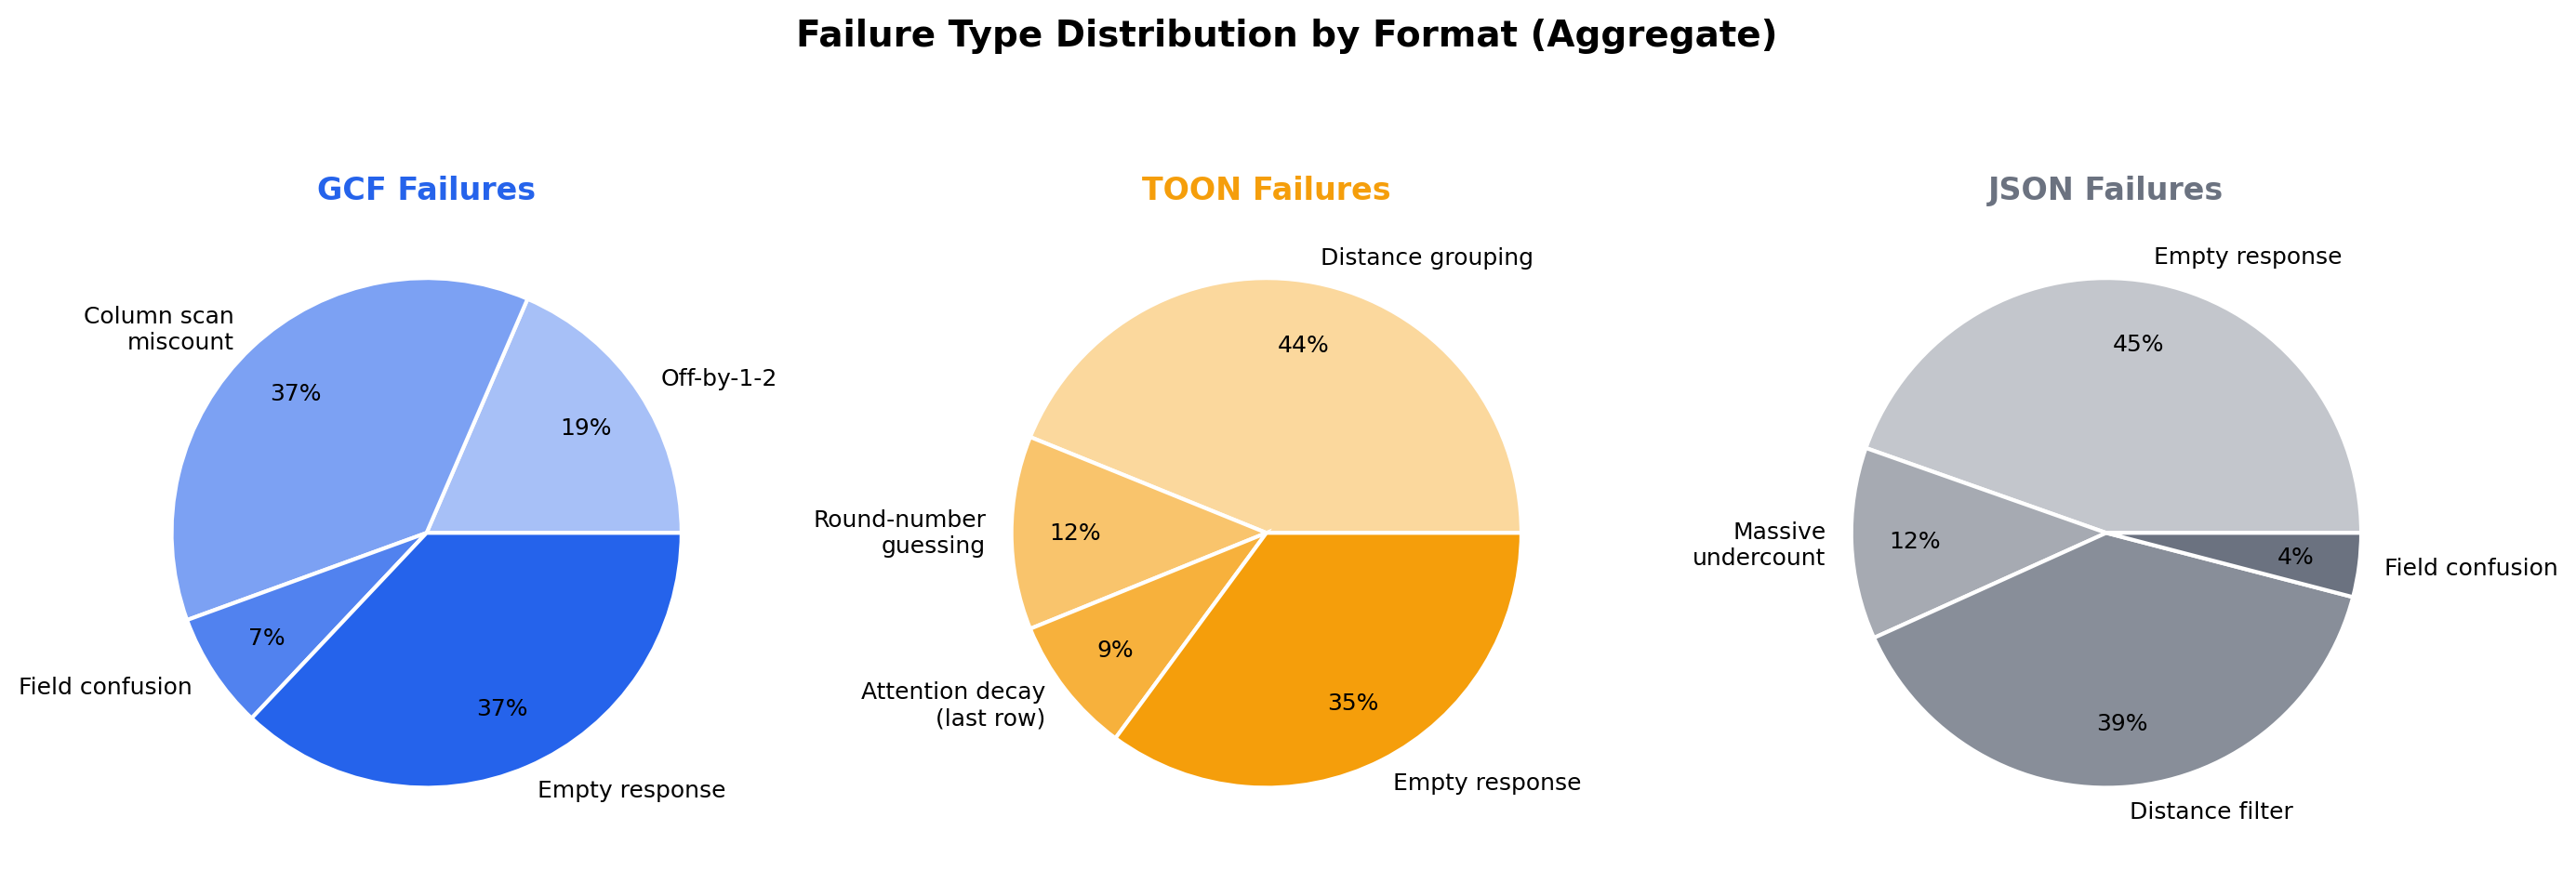
\includegraphics[keepaspectratio,alt={Failure Type Distribution}]{public/charts/failure-types-pie.png}}
\caption{Failure Type Distribution}
\end{figure}

\begin{figure}
\centering
\pandocbounded{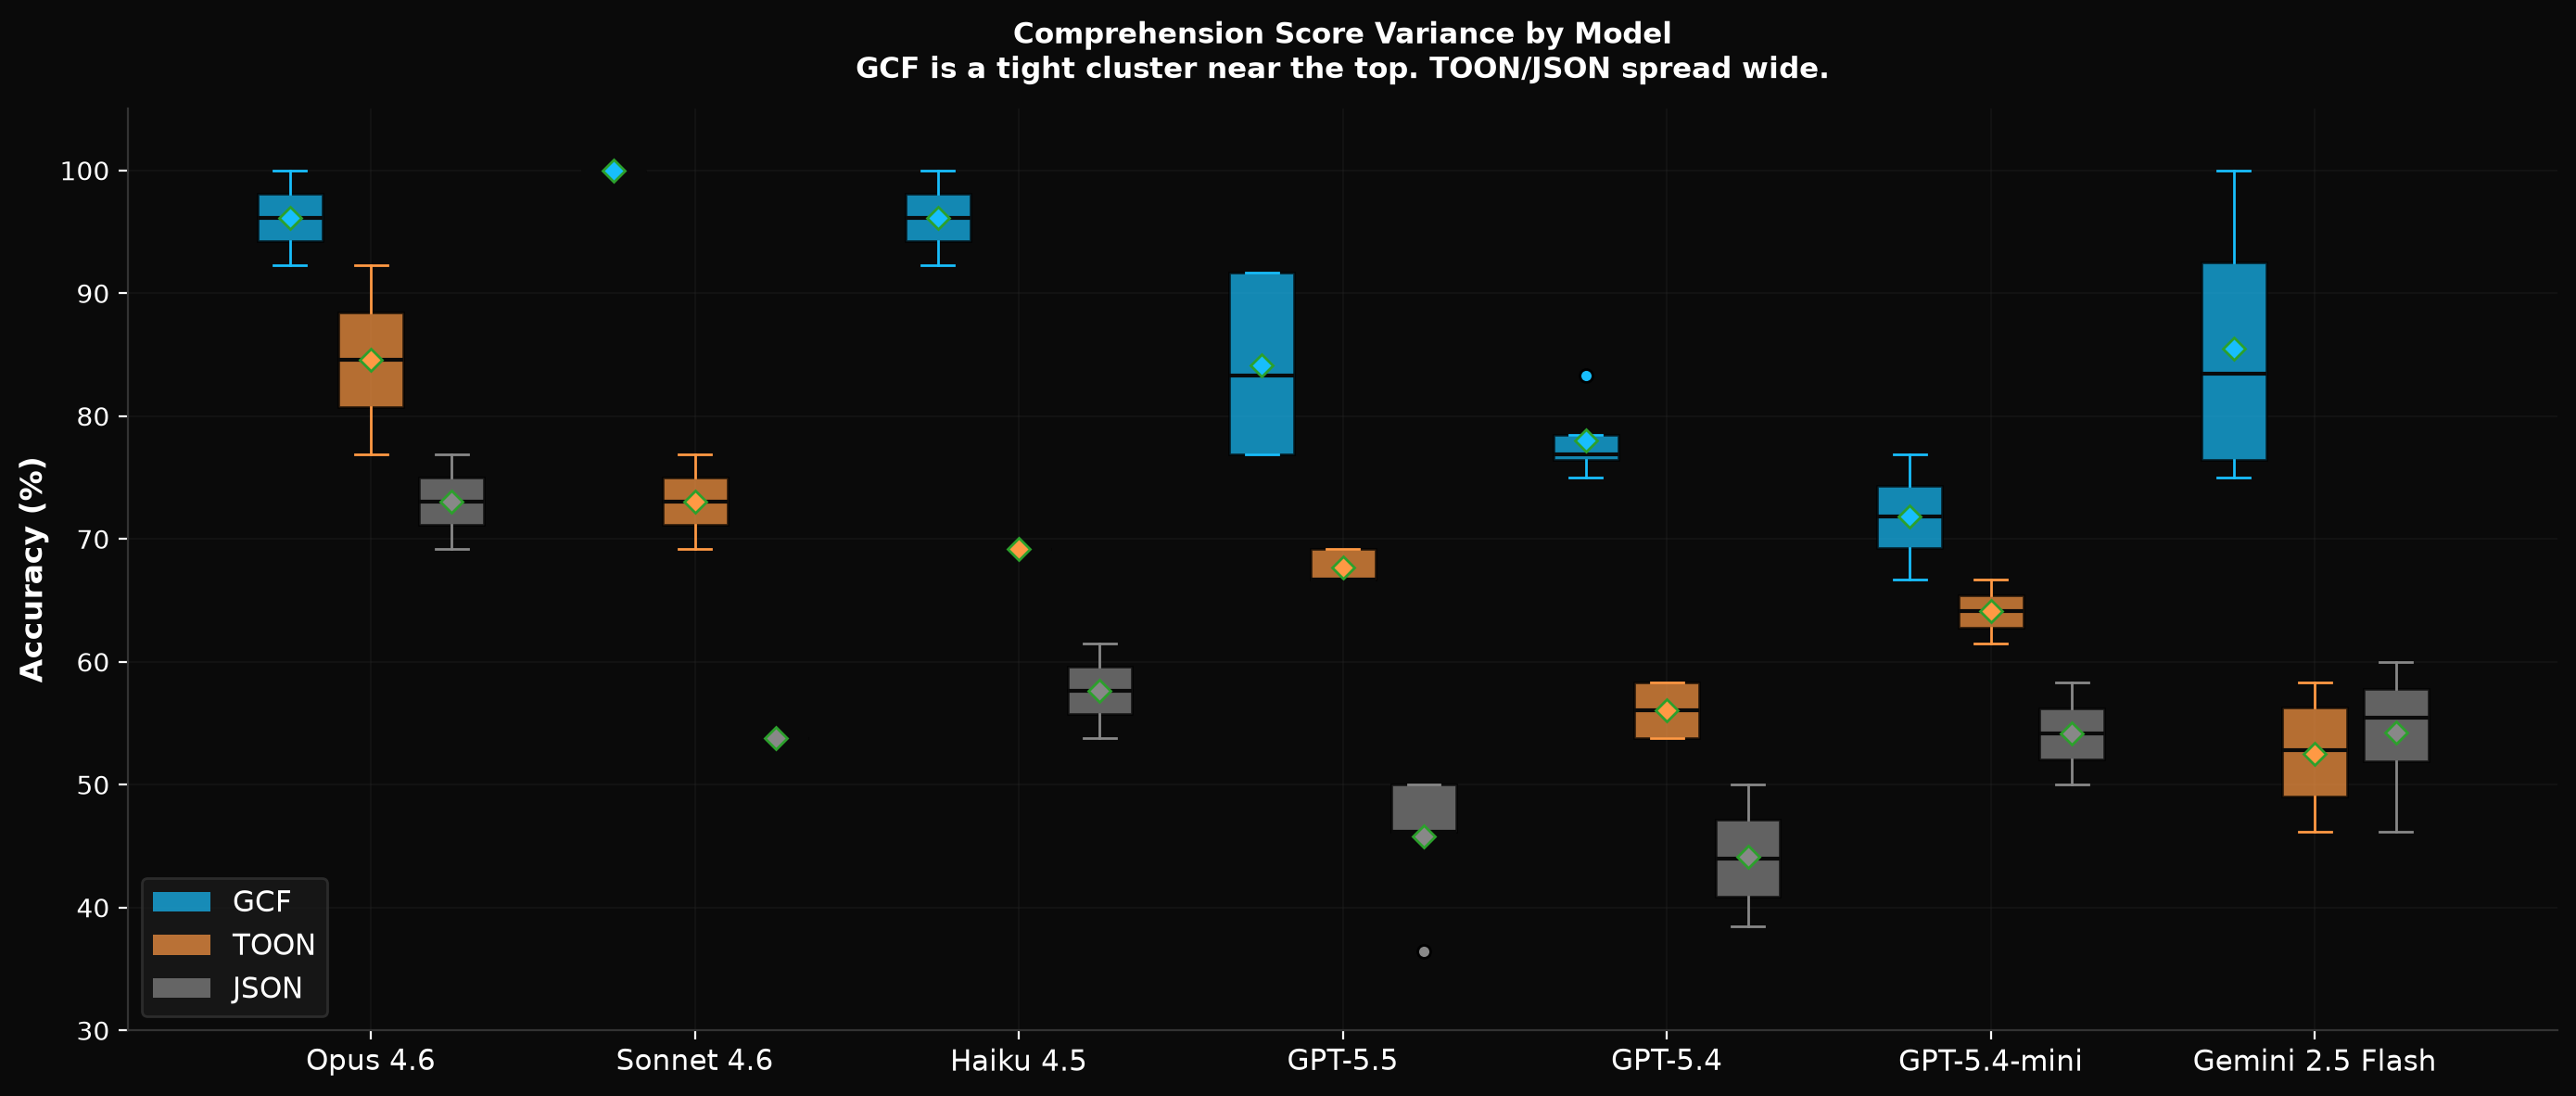
\includegraphics[keepaspectratio,alt={Comprehension Score Variance}]{public/charts/comprehension-variance.png}}
\caption{Comprehension Score Variance}
\end{figure}

\begin{figure}
\centering
\pandocbounded{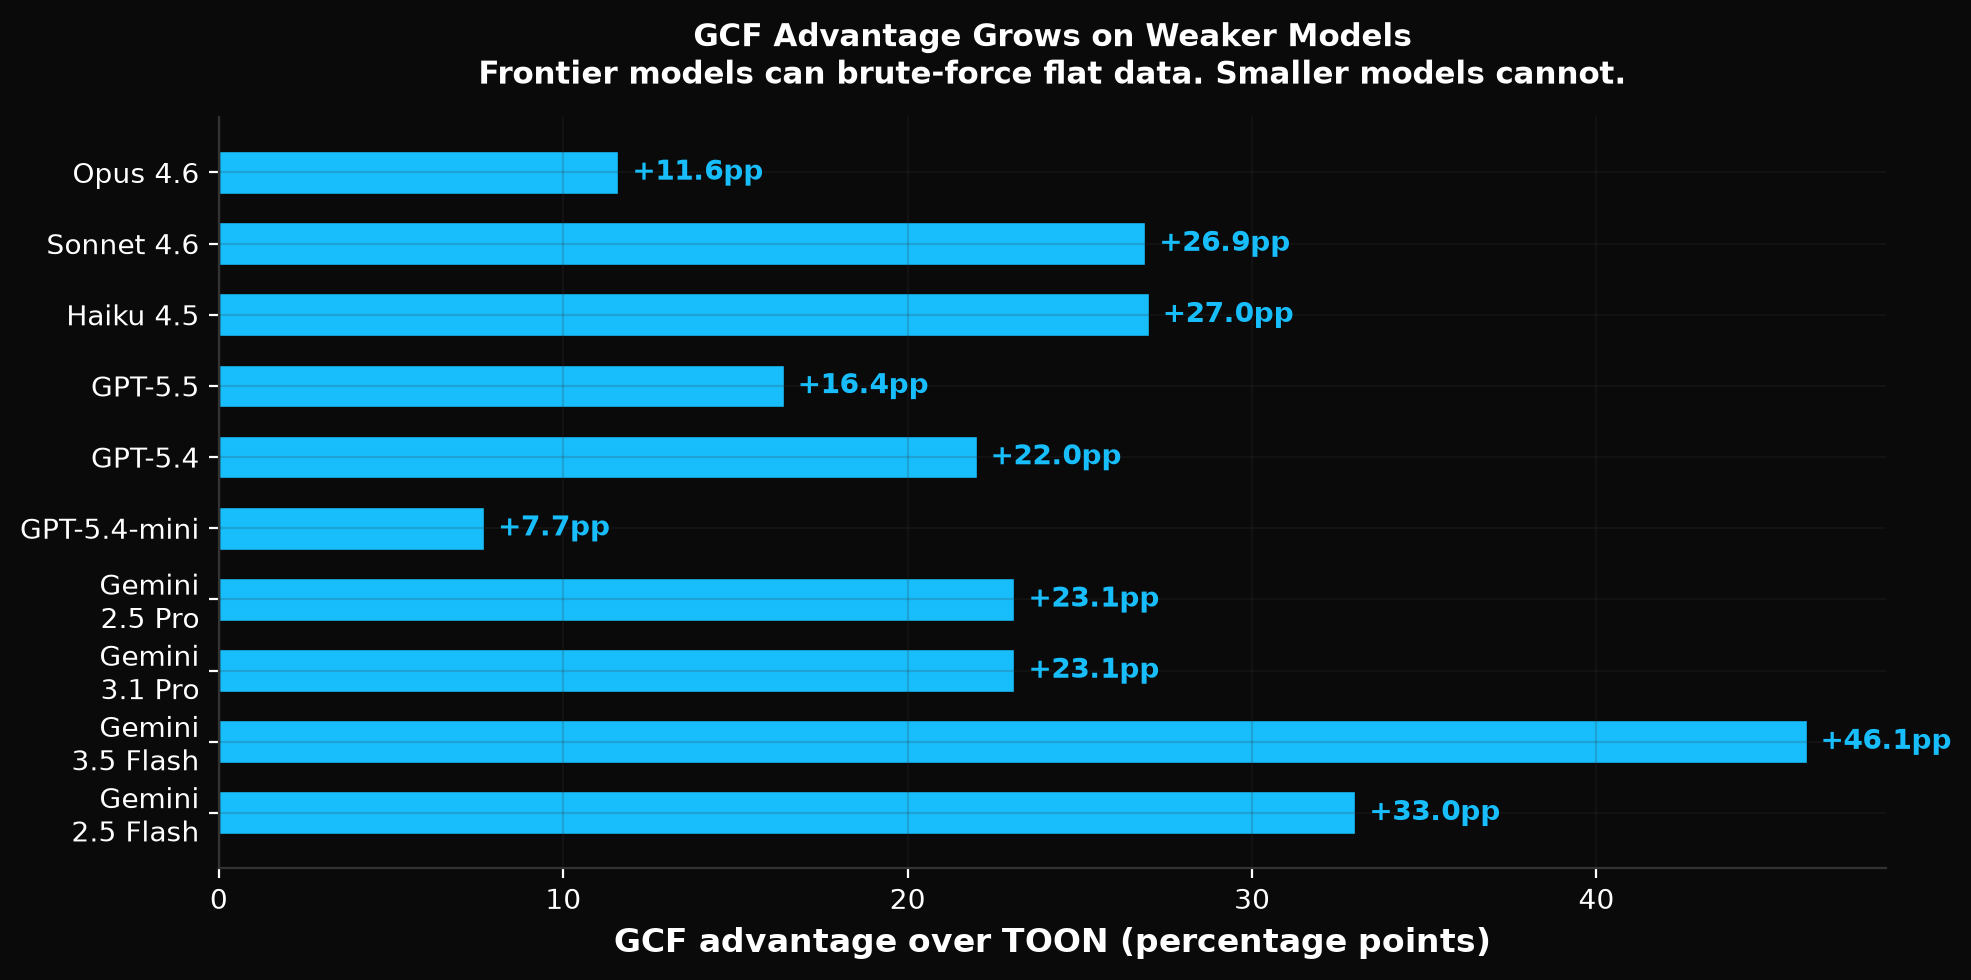
\includegraphics[keepaspectratio,alt={GCF Advantage Grows on Weaker Models}]{public/charts/advantage-by-tier.png}}
\caption{GCF Advantage Grows on Weaker Models}
\end{figure}

\paragraph{Comprehension methodology}\label{comprehension-methodology}

\begin{itemize}
\tightlist
\item
  OpenAI runs used default temperature (non-zero).
  \texttt{EVAL\_TEMPERATURE=0} available for deterministic runs.
\item
  Claude evals via \texttt{claude\ -p} CLI with \texttt{-\/-model} flag.
\item
  OpenAI evals via chat completions API with exponential backoff on
  429s.
\item
  Google evals via generativelanguage API with retry logic.
\item
  TOON encoding uses the official \texttt{toon-go} library from the
  \texttt{toon-format} GitHub organization.
\item
  All raw logs in \texttt{eval/results/comprehension/}.
\end{itemize}

\subsubsection{6.2 Session Statefulness
Savings}\label{session-statefulness-savings}

{\def\LTcaptype{none} % do not increment counter
\begin{longtable}[]{@{}
  >{\raggedright\arraybackslash}p{(\linewidth - 8\tabcolsep) * \real{0.0833}}
  >{\raggedright\arraybackslash}p{(\linewidth - 8\tabcolsep) * \real{0.1806}}
  >{\raggedright\arraybackslash}p{(\linewidth - 8\tabcolsep) * \real{0.2083}}
  >{\raggedright\arraybackslash}p{(\linewidth - 8\tabcolsep) * \real{0.1667}}
  >{\raggedright\arraybackslash}p{(\linewidth - 8\tabcolsep) * \real{0.3611}}@{}}
\toprule\noalign{}
\begin{minipage}[b]{\linewidth}\raggedright
Call
\end{minipage} & \begin{minipage}[b]{\linewidth}\raggedright
New symbols
\end{minipage} & \begin{minipage}[b]{\linewidth}\raggedright
Reused symbols
\end{minipage} & \begin{minipage}[b]{\linewidth}\raggedright
GCF tokens
\end{minipage} & \begin{minipage}[b]{\linewidth}\raggedright
Cumulative savings vs JSON
\end{minipage} \\
\midrule\noalign{}
\endhead
\bottomrule\noalign{}
\endlastfoot
1 & 10 & 0 & 233 & 75.9\% \\
2 & 5 & 4 & 128 & 82.3\% \\
3 & 3 & 6 & 87 & 86.1\% \\
4 & 2 & 7 & 62 & 89.4\% \\
5 & 1 & 8 & 41 & 92.7\% \\
\end{longtable}
}

By the fifth tool call in a session, GCF achieves 92.7\% token savings
versus JSON because 8 of 9 referenced symbols are bare ID references
(\texttt{@0}, \texttt{@3}) consuming 1 token each instead of 15-20
tokens for the full qualified name.

\begin{center}\rule{0.5\linewidth}{0.5pt}\end{center}

\begin{center}\rule{0.5\linewidth}{0.5pt}\end{center}

\subsection{7. Comparison to
Alternatives}\label{comparison-to-alternatives}

\subsubsection{7.1 Columnar/TSV}\label{columnartsv}

Column headers with tab-separated values eliminate field name
repetition, achieving \textasciitilde27\% token savings. But TSV treats
graph data as flat tables: edge references still require full identifier
strings in each row. TSV cannot exploit referential identity (local IDs)
or topological encoding (edge arrows). GCF triples the savings.

\subsubsection{7.2 Binary Formats (Protobuf, MessagePack,
FlatBuffers)}\label{binary-formats-protobuf-messagepack-flatbuffers}

These optimize for machine parsing and byte size. An LLM cannot read a
protobuf payload; it must be decoded to text first, and the decoded text
is typically JSON, eliminating the savings at the point of consumption.
Binary formats solve a different problem (machine efficiency) than GCF
(LLM token efficiency).

\subsubsection{7.3 JSON-LD / RDF}\label{json-ld-rdf}

Verbose by design: full URIs, type annotations, \texttt{@context}
declarations. Optimizes for semantic interoperability across systems,
not token-constrained consumption. JSON-LD is worse than JSON for LLM
tool responses.

\subsubsection{7.4 Markdown / Freeform
Text}\label{markdown-freeform-text}

Some tools return markdown-formatted text. This is human-optimized, not
LLM-optimized. Markdown uses whitespace for structure (indentation, line
breaks, headers) which tokenizers handle inconsistently. GCF's
positional format produces consistent, predictable token counts
regardless of tokenizer implementation.

\subsubsection{7.5 TOON (Token-Oriented Object
Notation)}\label{toon-token-oriented-object-notation}

TOON is a tabular encoding format for JSON that declares array fields
once and uses comma-separated rows. It achieves 30-60\% savings versus
JSON on flat tabular data.

\textbf{TOON:}

\begin{verbatim}
tool: example
symbols[3]{name,kind,score,distance}:
  pkg.Auth,function,0.9,0
  pkg.Server,function,0.7,1
  pkg.Cache,type,0.4,2
edges[1]{source,target,type}:
  pkg.Server,pkg.Auth,calls
\end{verbatim}

\textbf{GCF (same data):}

\begin{verbatim}
GCF profile=graph tool=example symbols=3 edges=1
## targets
@0 fn pkg.Auth 0.90 lsp
## related
@1 fn pkg.Server 0.70 lsp
## extended
@2 type pkg.Cache 0.40 structural
## edges [1]
@0<@1 calls
\end{verbatim}

The structural difference: TOON puts all symbols in one flat table with
a \texttt{distance} column. GCF groups them into \texttt{\#\#\ targets},
\texttt{\#\#\ related}, \texttt{\#\#\ extended} sections. This
difference drives both the comprehension gap (models can't filter flat
tables at scale) and the generation gap (models write ``target'' instead
of 0 in TOON's distance column).

\textbf{Methodology:} We forked TOON's benchmark repository
(\texttt{github.com/toon-format/toon}), added GCF as one additional
formatter (a single file importing \texttt{encodeGeneric} from the
published \texttt{@blackwell-systems/gcf} npm package), and ran their
benchmark harness unchanged. Datasets, tokenizer (gpt-tokenizer,
o200k\_base), and methodology are entirely upstream. Results:

{\def\LTcaptype{none} % do not increment counter
\begin{longtable}[]{@{}llll@{}}
\toprule\noalign{}
Dataset & GCF & TOON & Result \\
\midrule\noalign{}
\endhead
\bottomrule\noalign{}
\endlastfoot
Semi-uniform event logs & 108,158 & 154,032 & \textbf{GCF 42\%
smaller} \\
E-commerce orders & 61,593 & 73,246 & \textbf{GCF 19\% smaller} \\
Employee records (flat) & 49,055 & 49,966 & \textbf{GCF 2\% smaller} \\
Analytics time-series & 8,398 & 9,127 & \textbf{GCF 8\% smaller} \\
GitHub repos & 8,576 & 8,744 & \textbf{GCF 2\% smaller} \\
Deeply nested config & 616 & 618 & \textbf{GCF 0.3\% smaller} \\
\end{longtable}
}

\textbf{GCF wins all 6 datasets.} TOON has no token efficiency advantage
on any data shape.

TOON has no local-ID system, no edge encoding, no session deduplication,
no delta encoding, and no streaming mode. These are structural
limitations that cannot be added without a fundamental redesign. TOON
edges must repeat the full qualified name of both source and target
(\textasciitilde100 tokens per edge vs \textasciitilde4 for GCF). TOON
retransmits every record on every call; GCF tracks what's been sent.
TOON's spec mandates upfront \texttt{{[}N{]}} counts with no deferred
mechanism; GCF streams with zero buffering.

\textbf{TOON is fundamentally fragile for generation.} Its official
decoder rejects LLM-generated output on 7 of 9 models tested. The
failure is always the same: models write semantic labels where TOON
expects integers. This is a structural design flaw in flat tabular
formats that encode categories as column values. GCF solves this by
expressing categories through section placement. See Section 9.1 for the
full analysis.

On output, GCF produces 63\% smaller output than JSON and 33\% smaller
than TOON at 100 symbols.

Fork with reproducible results: github.com/blackwell-systems/toon
(branch: gcf-comparison).

\subsubsection{7.6 Custom Compressed JSON}\label{custom-compressed-json}

JSON with shortened field names (\texttt{"qn"} instead of
\texttt{"qualified\_name"}) achieves 15-25\% savings. This preserves
JSON's structural overhead (delimiters, quoting, nesting) while reducing
readability. GCF eliminates the structural overhead entirely rather than
shortening the labels on it.

\begin{center}\rule{0.5\linewidth}{0.5pt}\end{center}

\subsection{8. Limitations and
Validation}\label{limitations-and-validation}

\textbf{LLM comprehension.} 23 runs across 10 models and 3 providers
validate this design. GCF averages 90.7\% accuracy where JSON averages
53.6\% and TOON averages 68.5\%. Four models achieve 100\% on GCF. The
concern that LLMs might struggle with GCF's dense positional format was
unfounded; the format improves comprehension by eliminating structural
noise. GCF's \texttt{@N} local IDs, \texttt{\#\#} section headers, and
\texttt{\textbar{}} pipe separators are more comprehensible to an LLM
than JSON's \texttt{"qualified\_name":} repeated 500 times.

\textbf{LLM generation.} 28 generation runs across 9 models and 3
providers. GCF achieves 5/5 validity on every frontier model (Opus,
Sonnet, GPT-5.5, Gemini 2.5 Pro, Gemini 3.1 Pro) with a 3-line primer
and zero prior training. TOON's official decoder rejects LLM-generated
output on 7 of 9 models. The failure is structural: TOON's flat columns
encode semantic categories as integers, and models write labels
(``target'') instead of the expected integer (0). GCF expresses
categories through section placement (\texttt{\#\#\ targets}), aligning
with how models naturally express grouped data. GCF output is 63\%
smaller than JSON and 33\% smaller than TOON.

\textbf{Two profiles.} The graph profile is optimized for typed nodes
and edges. The generic profile (\texttt{encodeGeneric}) handles
arbitrary structured data (arrays of objects, nested records, mixed
types). On TOON's own benchmark with their datasets and tokenizer, GCF's
generic profile wins all 6 datasets. Primitive array inlining
(\texttt{name{[}N{]}:\ val1,val2,val3}) eliminated TOON's single
remaining advantage on deeply nested config.

\textbf{Session statefulness requires coordination.} The session ID
system assumes the server tracks which nodes have been transmitted to
which client. Stateless deployments cannot use session compression. The
non-session mode (full retransmission) remains available.

\textbf{Tokenizer dependency.} Token counts depend on the tokenizer. The
benchmarks in this paper use o200k\_base. Different tokenizers produce
different token counts for the same GCF payload, though the relative
savings versus JSON are consistent (within 2-3 percentage points).

\begin{center}\rule{0.5\linewidth}{0.5pt}\end{center}

\subsection{9. Implications for MCP and Agent
Tooling}\label{implications-for-mcp-and-agent-tooling}

The MCP specification does not define a standard for tool response
encoding beyond ``the response is a JSON-RPC result.'' This means every
MCP server independently decides how to format its output. The result is
that agents receive verbose JSON from every tool, with no mechanism to
request compact encoding.

We propose that MCP tool responses should support format negotiation:
the client specifies a preferred encoding in the tool call, and the
server returns the response in that encoding. GCF (or a format like it)
should be available as a standard option alongside JSON.

The token savings are too large to ignore. A 79\% reduction in tool
response tokens translates directly to: lower API costs, faster
time-to-first-token, more room in the context window for source code and
reasoning, and fewer multi-turn loops caused by context window
exhaustion.

\subsubsection{9.1 LLM Generation: GCF as a Bidirectional
Format}\label{llm-generation-gcf-as-a-bidirectional-format}

GCF is bidirectional: LLMs can produce it, not just consume it. 28
generation runs across 9 models and 3 providers, validated through real
decoders (including TOON's official \texttt{toon-go} library).

{\def\LTcaptype{none} % do not increment counter
\begin{longtable}[]{@{}llll@{}}
\toprule\noalign{}
Model & GCF & TOON (natural) & JSON \\
\midrule\noalign{}
\endhead
\bottomrule\noalign{}
\endlastfoot
Claude Opus 4.6 & \textbf{5/5} & 0/5 & 5/5 \\
Claude Sonnet 4.6 & \textbf{5/5} & 2-3/5 & 5/5 \\
Claude Haiku 4.5 & \textbf{5/5} & 1-3/5 & 5/5 \\
GPT-5.5 & \textbf{4-5/5} & 1-2/5 & 5/5 \\
GPT-5.4 & \textbf{5/5} & 0/5 & 5/5 \\
GPT-5.4-mini & \textbf{5/5} & 0/5 & 5/5 \\
Gemini 2.5 Pro & \textbf{5/5} & 1/5 & 5/5 \\
Gemini 3.1 Pro & \textbf{5/5} & 0/5 & 5/5 \\
Gemini 3.1 Flash Lite & \textbf{4-5/5} & 0/5 & 4-5/5 \\
\end{longtable}
}

\textbf{GCF 5/5 on every frontier model. TOON fails on 7 of 9 models.}

\begin{figure}
\centering
\pandocbounded{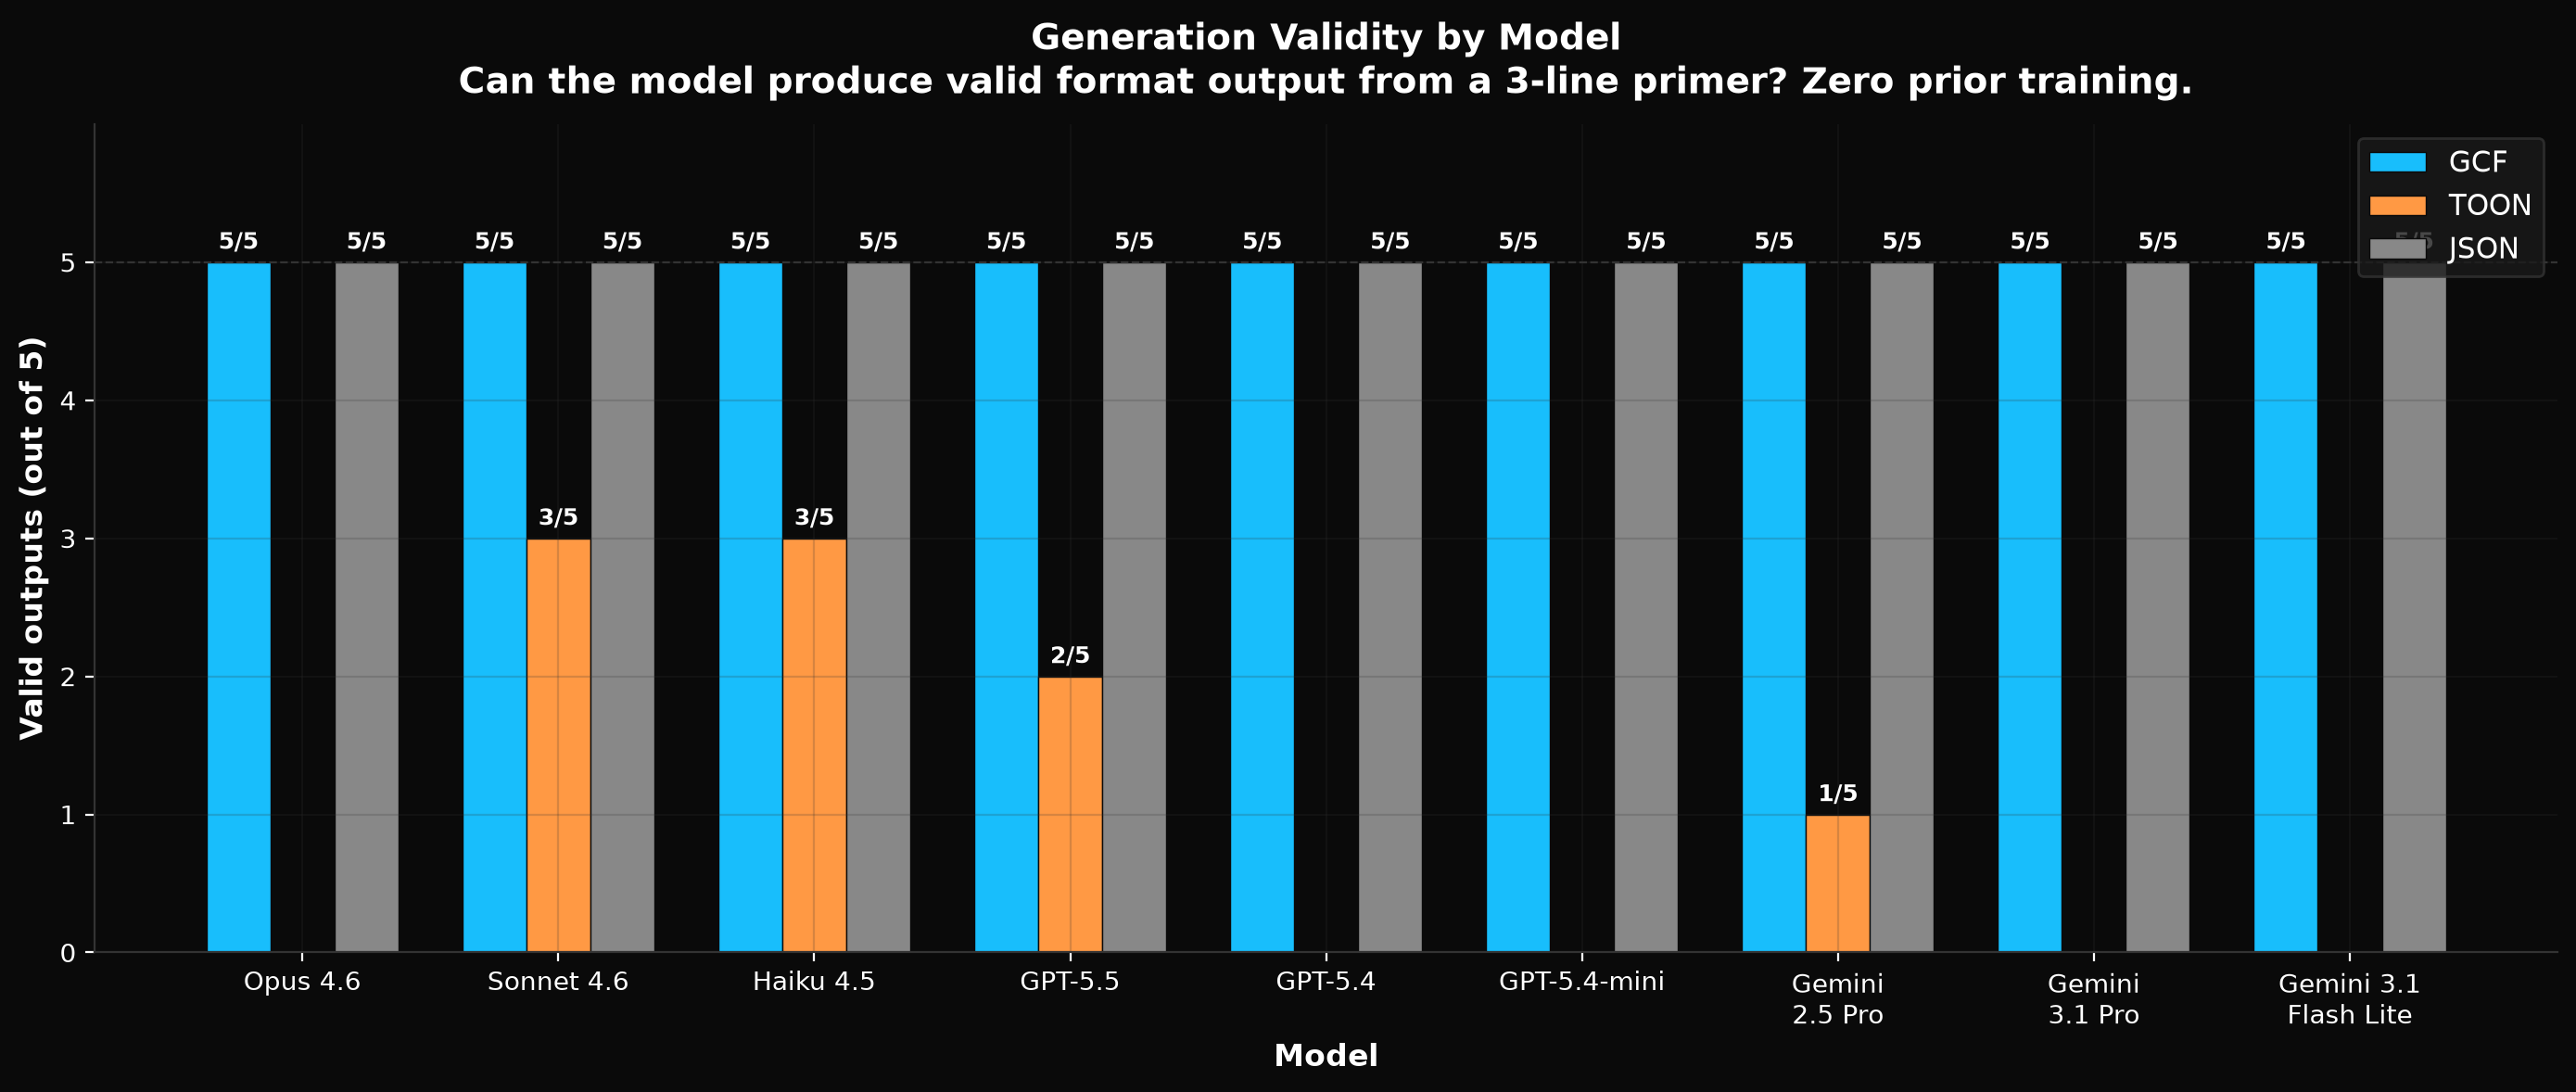
\includegraphics[keepaspectratio,alt={Generation Validity by Model}]{public/charts/generation-validity.png}}
\caption{Generation Validity by Model}
\end{figure}

\paragraph{Why TOON fails generation}\label{why-toon-fails-generation}

TOON's flat tabular design encodes semantic categories as column values.
When told ``this symbol is a target,'' the model writes \texttt{target}
in the distance column. TOON's decoder expects \texttt{0}. The model
would need to know, unprompted, that ``target'' maps to 0, ``related''
maps to 1, ``extended'' maps to 2. No model does this. The error is
always the same: \texttt{toon:\ cannot\ assign\ string\ to\ int}.

This is a structural design flaw in flat tabular formats. Any time a
column encodes a semantic category as an integer, the format is one
prompt change away from producing invalid data. TOON is fundamentally
fragile for LLM generation.

GCF expresses categories through section placement
(\texttt{\#\#\ targets}, \texttt{\#\#\ related}). The model writes the
symbol in the section matching the label. No integer mapping required.
The format aligns with how LLMs naturally express grouped data.

\begin{figure}
\centering
\pandocbounded{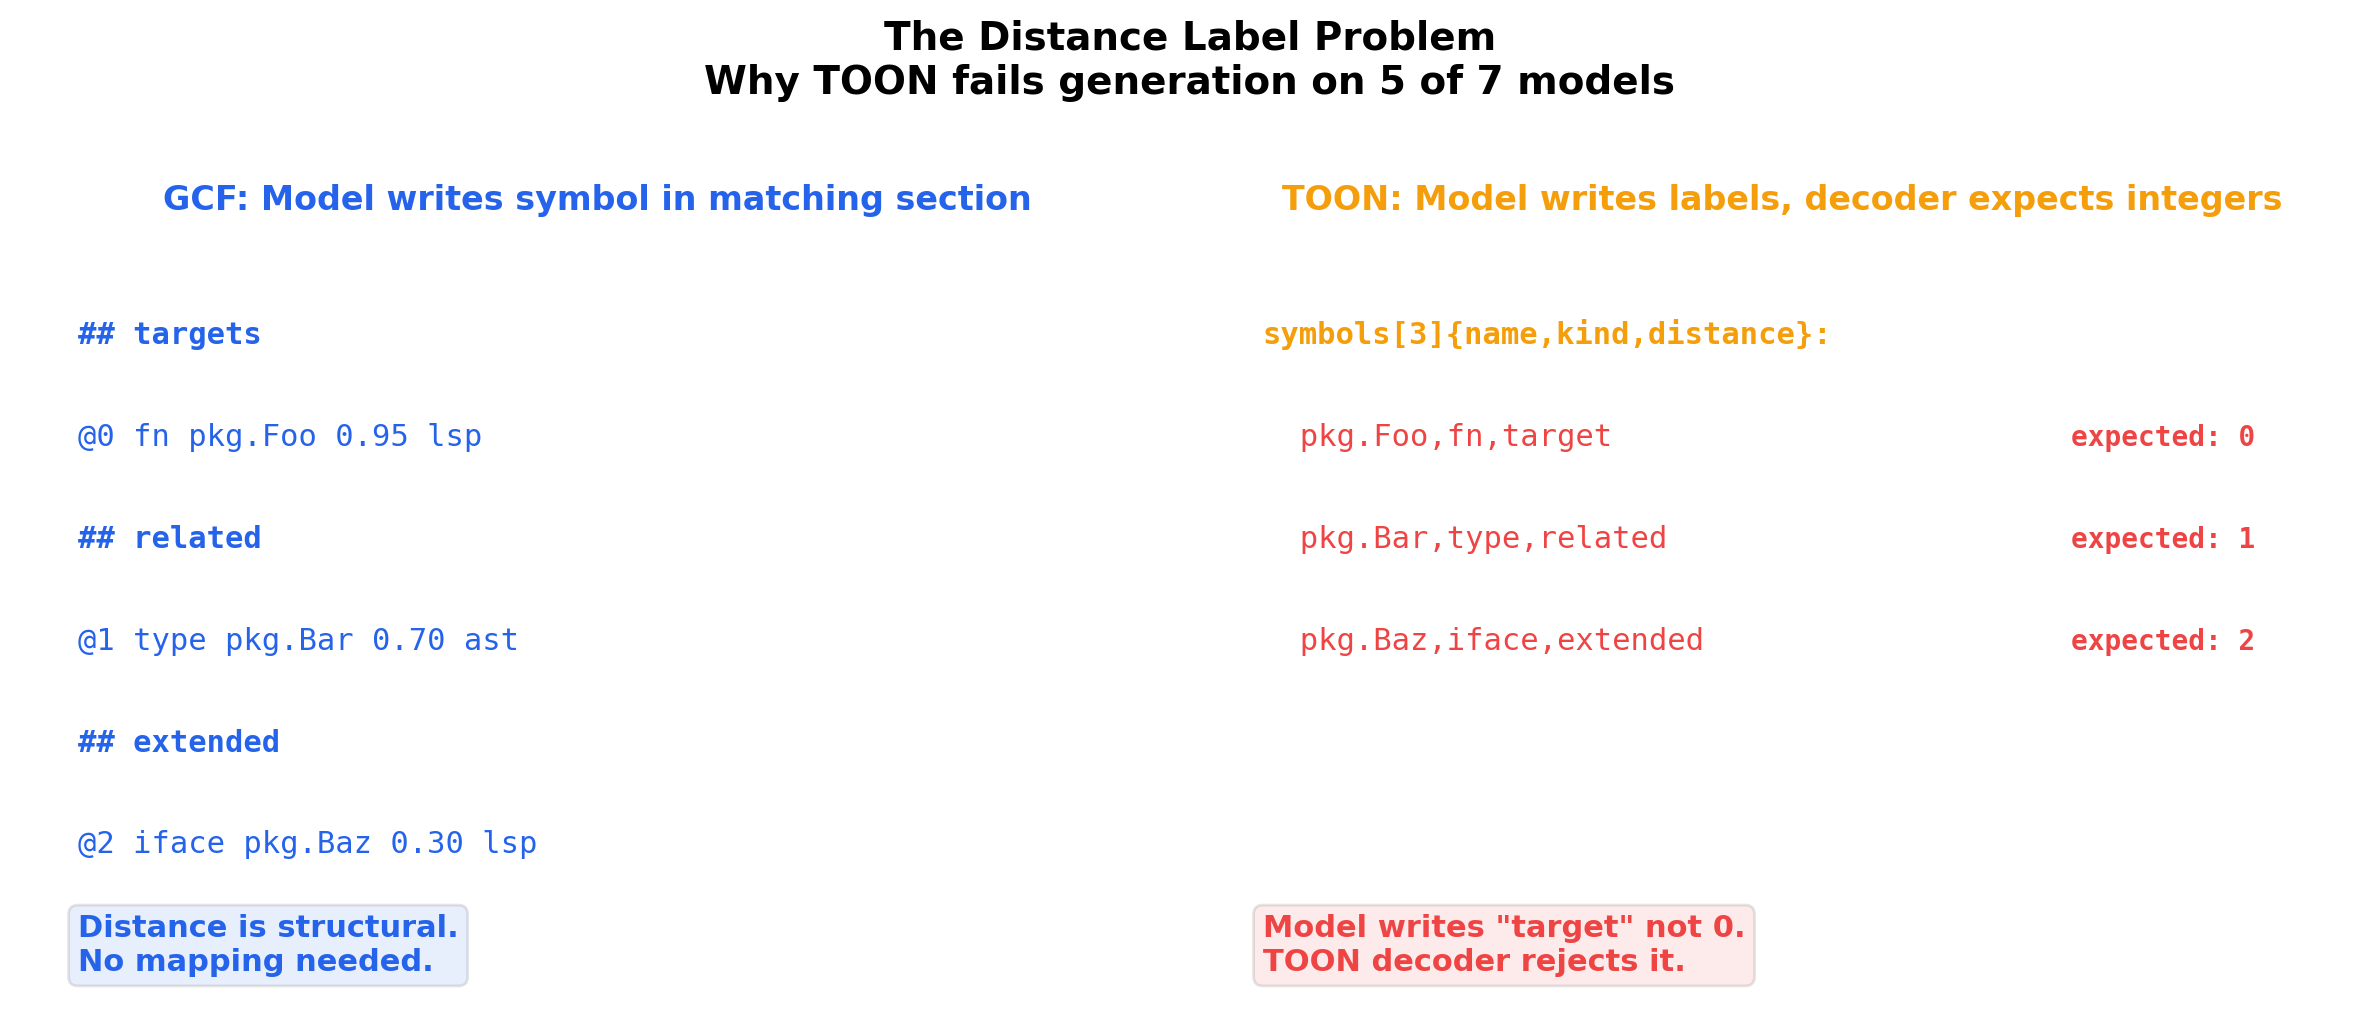
\includegraphics[keepaspectratio,alt={The Distance Label Problem}]{public/charts/distance-label-problem.png}}
\caption{The Distance Label Problem}
\end{figure}

\begin{figure}
\centering
\pandocbounded{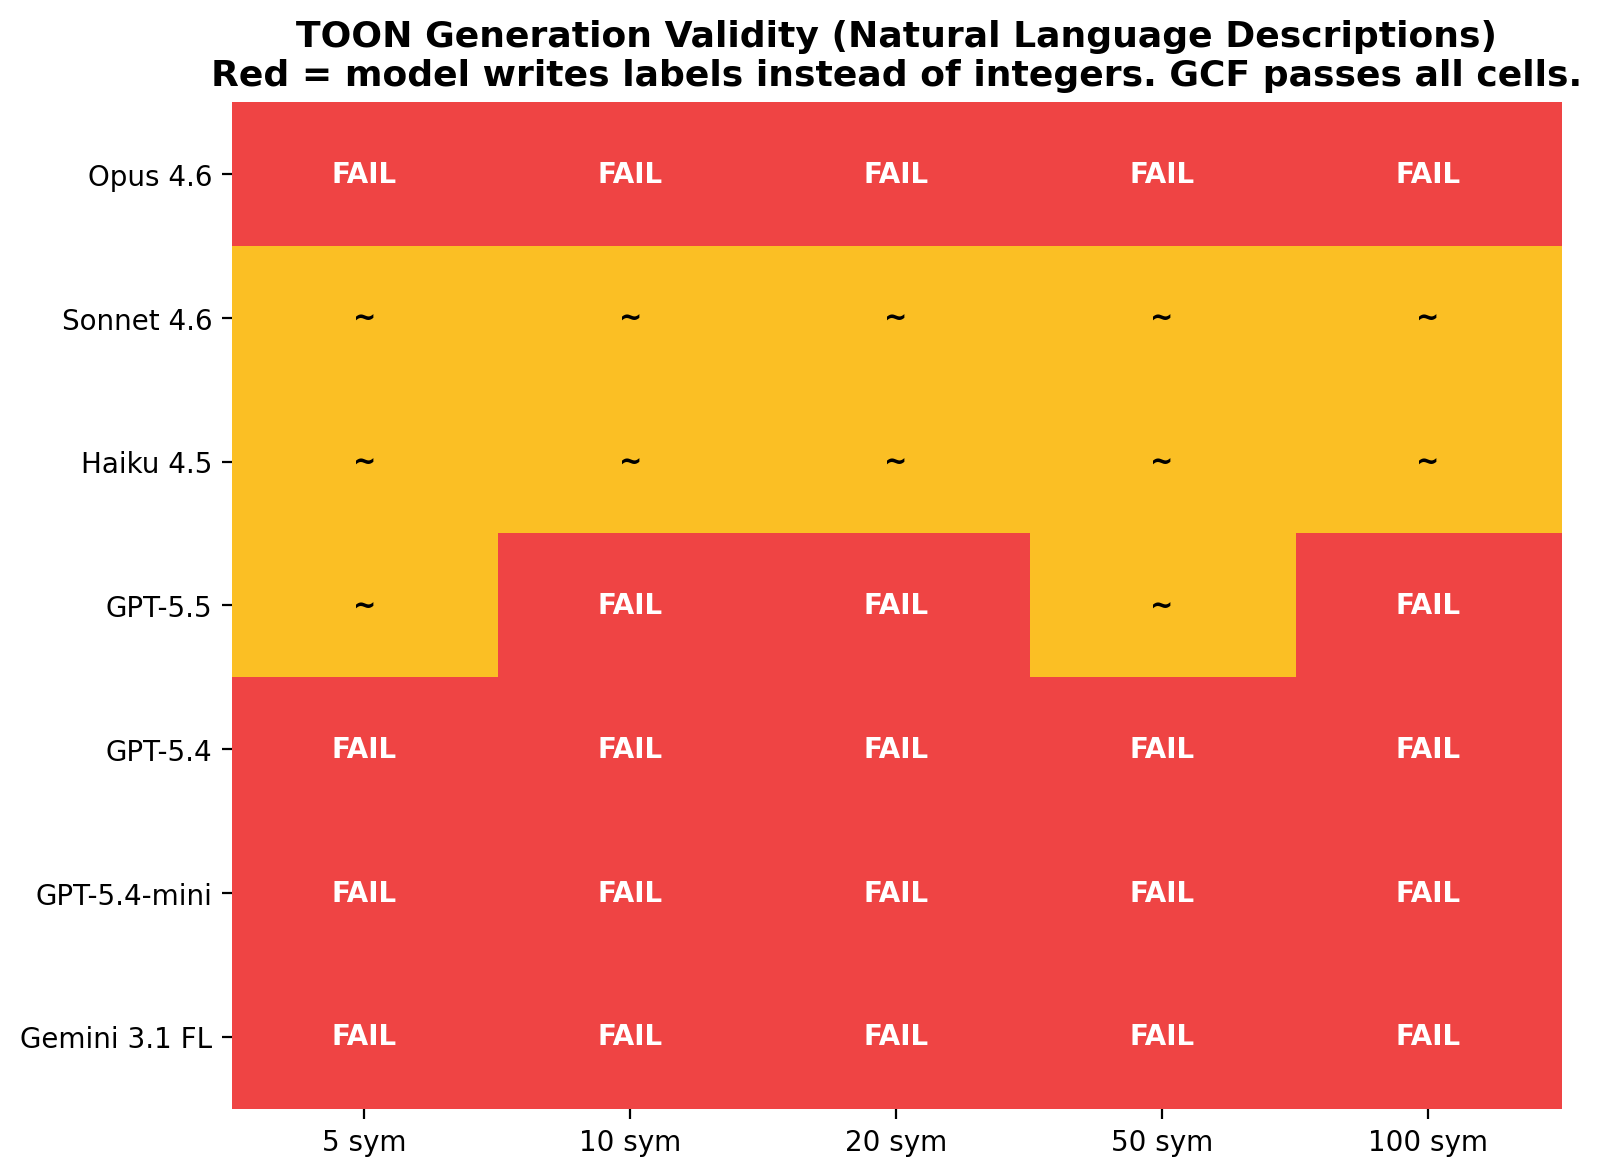
\includegraphics[keepaspectratio,alt={TOON Generation Heatmap}]{public/charts/toon-heatmap.png}}
\caption{TOON Generation Heatmap}
\end{figure}

When TOON is given pre-encoded integers (hand-holding the model through
the mapping), performance improves on some models but remains
inconsistent. Even in the best case, GCF output is 28\% smaller.

\paragraph{Output size comparison}\label{output-size-comparison}

{\def\LTcaptype{none} % do not increment counter
\begin{longtable}[]{@{}lll@{}}
\toprule\noalign{}
Format & 100 sym output & vs JSON \\
\midrule\noalign{}
\endhead
\bottomrule\noalign{}
\endlastfoot
\textbf{GCF} & \textbf{5,976 B} & \textbf{63\% fewer} \\
TOON & 8,937 B & 45\% fewer \\
JSON & 16,121 B & baseline \\
\end{longtable}
}

\begin{figure}
\centering
\pandocbounded{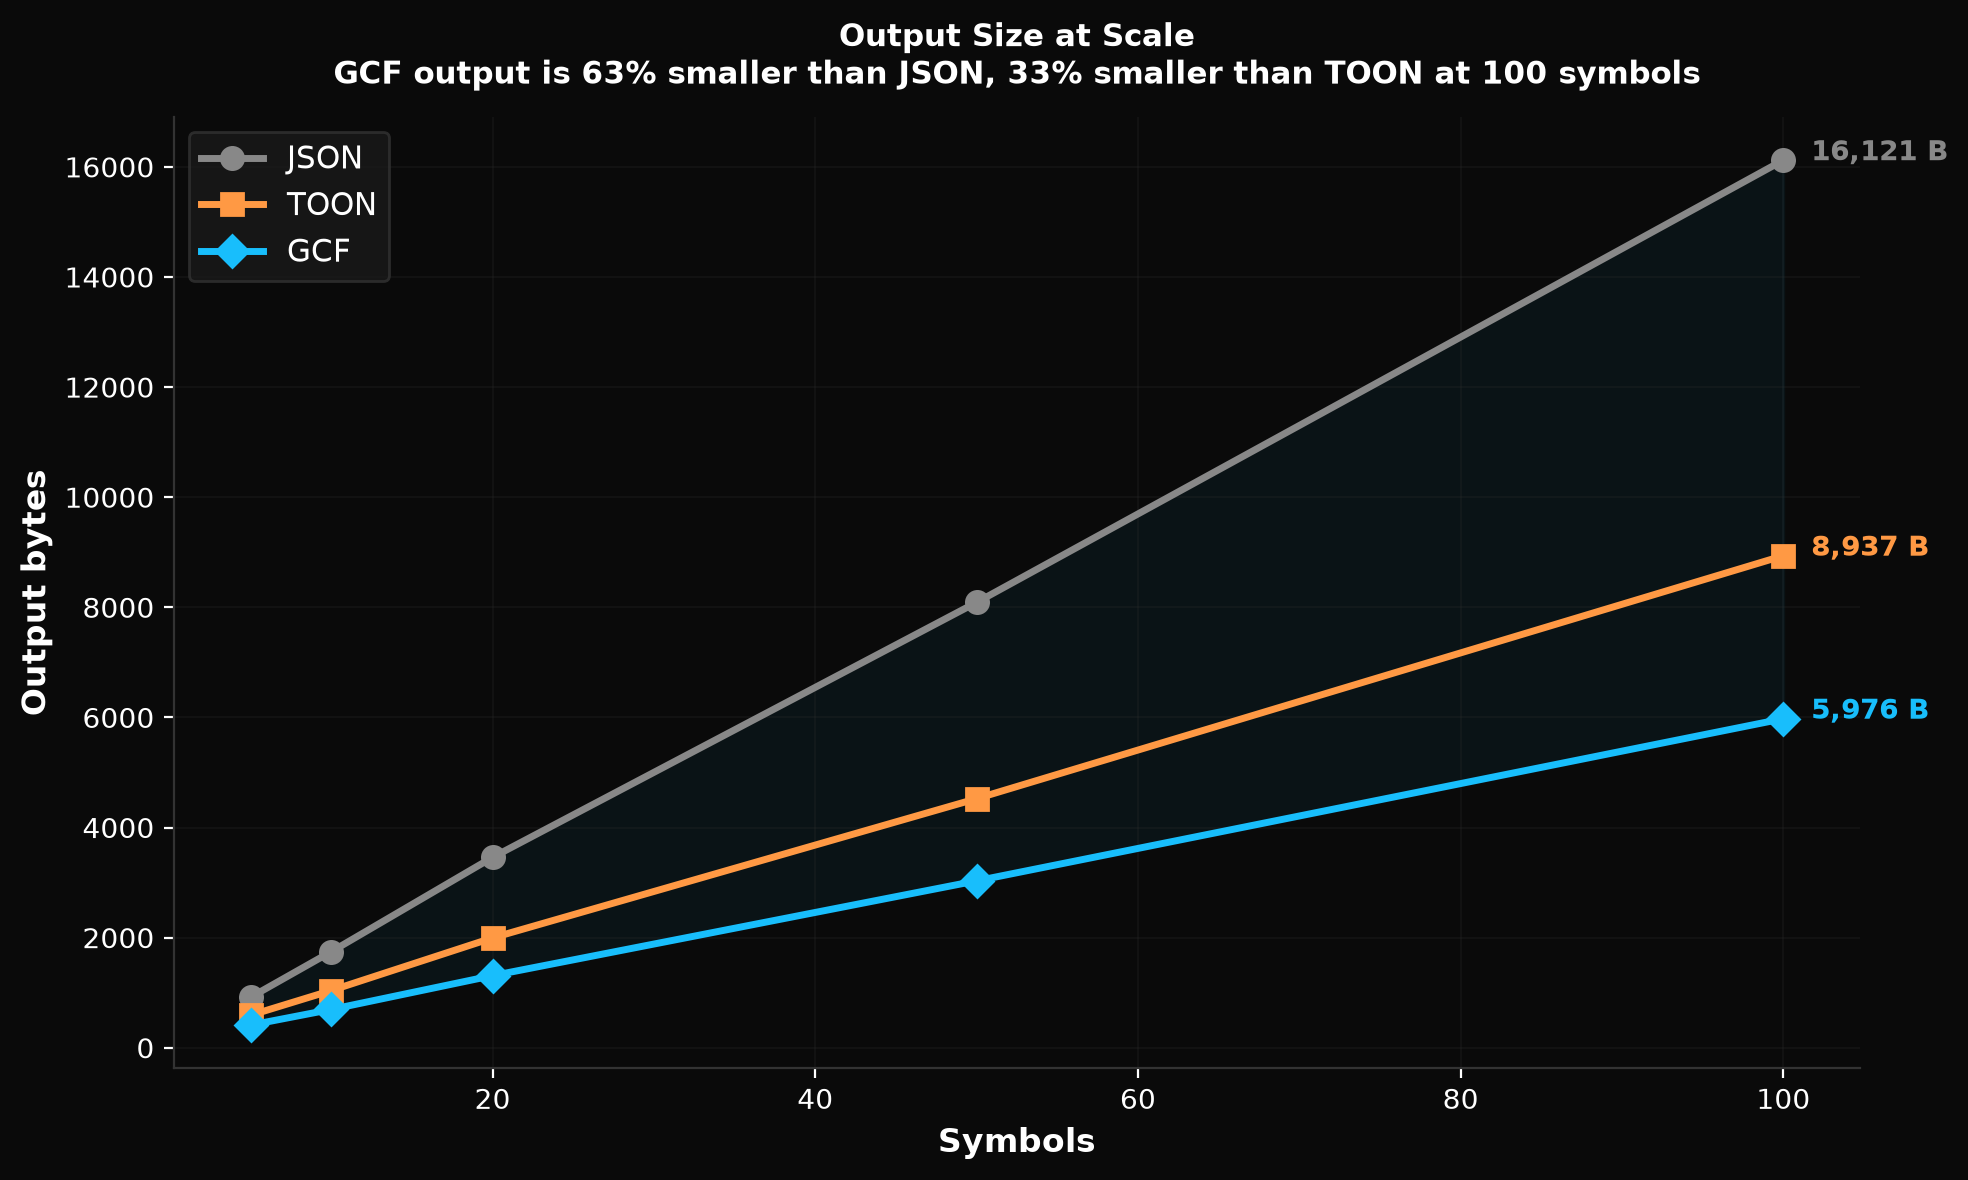
\includegraphics[keepaspectratio,alt={Output Size at Scale}]{public/charts/output-cost-at-scale.png}}
\caption{Output Size at Scale}
\end{figure}

\textbf{Implications.} GCF generation enables: (1) agent-to-agent
communication at 63\% fewer tokens per handoff, (2) structured output
mode as an alternative to JSON mode, and (3) system prompt encoding
where context packs are encoded as GCF to maximize context window
utilization.

\subsubsection{9.2 Streaming: Progressive Context
Delivery}\label{streaming-progressive-context-delivery}

The streaming encoding extension (Section 3.8) enables a new interaction
pattern: \textbf{progressive context delivery}. An MCP proxy can emit
GCF fragments as MCP progress notifications while the upstream server is
still processing. The LLM receives partial context immediately, reducing
perceived latency from seconds to milliseconds on large graph
traversals.

Combined with MCP's Streamable HTTP transport (Server-Sent Events), this
creates a pipeline where graph data flows from the server through the
proxy to the LLM token by token, with the trailer summary providing
count verification at the end.

\subsubsection{9.3 Delta Encoding}\label{delta-encoding}

GCF's token savings compound with delta encoding: when the agent passes
a \texttt{pack\_root} from a prior call and the pack changed, the server
sends only added/removed symbols instead of the full payload. Measured:
81.2\% additional token savings at 96.6\% symbol overlap on re-query
scenarios. Combined with GCF's baseline savings and session
deduplication, the three-level stack achieves over 97\% cumulative token
reduction on warm sessions versus stateless JSON.

\begin{center}\rule{0.5\linewidth}{0.5pt}\end{center}

\subsection{10. Conclusion}\label{conclusion}

JSON is the default encoding for LLM interactions because it is
universal, not because it is efficient. For structured data, JSON wastes
more than three-quarters of its tokens on structural overhead that
carries no semantic content.

GCF eliminates this waste through two encoding profiles. The graph
profile uses referential identity (local IDs), topological encoding
(edge arrows), and hierarchical grouping (section headers) for code
graph data. The generic profile uses positional rows with pipe
separators, section headers, and inline primitive arrays for arbitrary
structured data. Both achieve significant savings: 79\% versus JSON on
graph data at 500 symbols, 34\% versus TOON on TOON's own
mixed-structure benchmark (winning all 6 datasets).

GCF is bidirectional. 1,300+ LLM evaluations across 10 models and 3
providers prove it. Comprehension: 90.7\% average accuracy (four models
at 100\%) where JSON averages 53.6\% and TOON averages 68.5\%.
Generation: 5/5 validity on every frontier model where TOON fails on 7
of 9 models. Output: 63\% fewer tokens than JSON, 33\% fewer than TOON.
Session deduplication (92.7\% by the fifth call), delta encoding (81.2\%
on re-queries), and streaming encode (zero-buffering with trailer
summary) compound savings across multi-turn interactions. No competing
format offers these features.

The format is text-based, LLM-optimized, and implementable in any
language. Implementations exist in six languages (Go, TypeScript,
Python, Rust, Swift, Kotlin), all at v1.0.0+ with CLIs, zero or minimal
runtime dependencies, and 200M+ verified lossless round-trips. A
bidirectional MCP proxy enables adoption with zero code changes: session
dedup (40\% savings proven e2e), proxy-level delta encoding (68\%
savings on incremental changes), HTTP backend/frontend for remote
deployment, response caching, and streaming progress notifications. JSON
Schema validation works on decoded output unchanged, eliminating the
primary enterprise adoption objection.

The broader point: GCF is a wire format. Wire formats are not optimized
for human readability. HTTP headers are not readable. Protobuf is not
readable. Nobody cares; they use a viewer. GCF is the wire format; JSON
is the viewer format. The agent reads GCF (cheap, accurate), does its
work, then calls \texttt{decode()} at the end if a human needs to see
the result. Human readability is a last-mile rendering concern, not a
wire format property.

The format that looks clean to humans (JSON) is the one that breaks for
agents at scale. The format optimized for agentic comprehension (GCF)
achieves 90.7\% average accuracy across 10 models at the lowest token
cost, with four models hitting 100\%. TOON, the format positioned as the
compromise between human readability and machine efficiency, fails
generation on 7 of 9 models and never achieves 100\% comprehension on
any model. This is not a tradeoff. It is a design choice validated by
1,300+ evaluations across every major AI provider.

\begin{center}\rule{0.5\linewidth}{0.5pt}\end{center}

\subsection{Reference Implementation}\label{reference-implementation}

\begin{itemize}
\tightlist
\item
  \textbf{Specification:} gcformat.com (v2.0 Stable, RFC 2119 keywords,
  conformance checklists, streaming extension, error taxonomy, i18n,
  status lifecycle)
\item
  \textbf{Go library:} \texttt{github.com/blackwell-systems/gcf-go}
  (v1.0.2). CLI: \texttt{gcf\ encode-generic},
  \texttt{gcf\ decode-generic}
\item
  \textbf{TypeScript library:} \texttt{@blackwell-systems/gcf} on npm
  (v1.0.1). CLI: \texttt{npx\ @blackwell-systems/gcf\ encode-generic}
\item
  \textbf{Python library:} \texttt{gcf-python} on PyPI (v1.0.1). CLI:
  \texttt{python\ -m\ gcf\ encode-generic}
\item
  \textbf{Rust library:} \texttt{gcf} on crates.io (v1.0.1). CLI:
  \texttt{gcf\ encode-generic}
\item
  \textbf{Swift library:} \texttt{gcf-swift} via SPM (v1.0.1). CLI:
  \texttt{swift\ run\ GCFCLI\ encode-generic}
\item
  \textbf{Kotlin library:} \texttt{gcf-kotlin} via JitPack (v1.0.1).
  CLI: \texttt{gradle\ run\ -\/-args="encode-generic"}
\item
  \textbf{MCP proxy:} \texttt{github.com/blackwell-systems/gcf-proxy}
  (v0.10.0): bidirectional translation, session dedup, delta encoding,
  HTTP backend/frontend, response caching, min-size bypass, streaming
  progress
\item
  \textbf{Comprehension eval:}
  \texttt{github.com/blackwell-systems/gcf-go/eval} (500 symbols, 13
  questions, 3 formats, 10 models, 3 providers)
\item
  \textbf{Generation eval:}
  \texttt{github.com/blackwell-systems/gcf-go/eval} (5-100 symbols, GCF
  vs TOON vs JSON, 9 models, validated through real decoders)
\item
  \textbf{Eval results:}
  \texttt{github.com/blackwell-systems/gcf/eval/results} (all raw logs,
  failure taxonomy, artifacts)
\item
  \textbf{TOON benchmark fork:}
  \texttt{github.com/blackwell-systems/toon} (branch: gcf-comparison,
  their datasets, their tokenizer)
\item
  \textbf{Conformance test suite:}
  \texttt{github.com/blackwell-systems/gcf/tests/conformance} (141 v2
  fixtures across both profiles, streaming, and normative errors)
\item
  \textbf{Cross-language matrix:}
  \texttt{github.com/blackwell-systems/gcf/tests/cross-language-matrix.py}
  (5x5 encode/decode verification)
\item
  \textbf{Schema validation guide:} gcformat.com/guide/schema-validation
  (JSON Schema on decoded output, three validation patterns)
\item
  \textbf{FAQ:} gcformat.com/guide/faq (protobuf, MessagePack, CBOR,
  gzip, YAML comparisons)
\item
  \textbf{Interactive playground:} gcformat.com/playground (three-way
  JSON vs TOON vs GCF comparison using real @toon-format/toon library)
\item
  \textbf{Production deployment:} knowing (28 MCP tools), agent-lsp (66
  MCP tools), NeuroNest (first independent commercial adoption)
\end{itemize}

\begin{center}\rule{0.5\linewidth}{0.5pt}\end{center}

\subsection{Appendix A: Full Example}\label{appendix-a-full-example}

\textbf{JSON (965 tokens):}

\begin{Shaded}
\begin{Highlighting}[]
\FunctionTok{\{}
  \DataTypeTok{"tool"}\FunctionTok{:} \StringTok{"context\_for\_task"}\FunctionTok{,}
  \DataTypeTok{"tokens\_used"}\FunctionTok{:} \DecValTok{1847}\FunctionTok{,}
  \DataTypeTok{"token\_budget"}\FunctionTok{:} \DecValTok{5000}\FunctionTok{,}
  \DataTypeTok{"symbols"}\FunctionTok{:} \OtherTok{[}
    \FunctionTok{\{}
      \DataTypeTok{"qualified\_name"}\FunctionTok{:} \StringTok{"github.com/blackwell{-}systems/knowing/internal/mcp.requireHash"}\FunctionTok{,}
      \DataTypeTok{"kind"}\FunctionTok{:} \StringTok{"function"}\FunctionTok{,}
      \DataTypeTok{"score"}\FunctionTok{:} \FloatTok{0.78}\FunctionTok{,}
      \DataTypeTok{"signature"}\FunctionTok{:} \StringTok{"func requireHash(args map[string]any, key string) (types.Hash, error)"}\FunctionTok{,}
      \DataTypeTok{"provenance"}\FunctionTok{:} \StringTok{"lsp\_resolved"}\FunctionTok{,}
      \DataTypeTok{"distance"}\FunctionTok{:} \DecValTok{0}\FunctionTok{,}
      \DataTypeTok{"components"}\FunctionTok{:} \FunctionTok{\{} \DataTypeTok{"blast\_radius"}\FunctionTok{:} \FloatTok{0.40}\FunctionTok{,} \DataTypeTok{"confidence"}\FunctionTok{:} \FloatTok{0.25}\FunctionTok{,} \DataTypeTok{"recency"}\FunctionTok{:} \FloatTok{0.06}\FunctionTok{,} \DataTypeTok{"distance"}\FunctionTok{:} \FloatTok{0.15} \FunctionTok{\}}
    \FunctionTok{\}}\OtherTok{,}
    \FunctionTok{\{}
      \DataTypeTok{"qualified\_name"}\FunctionTok{:} \StringTok{"github.com/blackwell{-}systems/knowing/internal/mcp.NewServer"}\FunctionTok{,}
      \DataTypeTok{"kind"}\FunctionTok{:} \StringTok{"function"}\FunctionTok{,}
      \DataTypeTok{"score"}\FunctionTok{:} \FloatTok{0.54}\FunctionTok{,}
      \DataTypeTok{"provenance"}\FunctionTok{:} \StringTok{"lsp\_resolved"}\FunctionTok{,}
      \DataTypeTok{"distance"}\FunctionTok{:} \DecValTok{1}
    \FunctionTok{\}}
  \OtherTok{]}\FunctionTok{,}
  \DataTypeTok{"edges"}\FunctionTok{:} \OtherTok{[}
    \FunctionTok{\{}
      \DataTypeTok{"source"}\FunctionTok{:} \StringTok{"github.com/blackwell{-}systems/knowing/internal/mcp.NewServer"}\FunctionTok{,}
      \DataTypeTok{"target"}\FunctionTok{:} \StringTok{"github.com/blackwell{-}systems/knowing/internal/mcp.requireHash"}\FunctionTok{,}
      \DataTypeTok{"edge\_type"}\FunctionTok{:} \StringTok{"calls"}
    \FunctionTok{\}}
  \OtherTok{]}
\FunctionTok{\}}
\end{Highlighting}
\end{Shaded}

\textbf{GCF (233 tokens):}

\begin{verbatim}
GCF profile=graph tool=context_for_task budget=5000 tokens=1847 symbols=2 edges=1
## targets
@0 fn github.com/blackwell-systems/knowing/internal/mcp.requireHash 0.78 lsp_resolved
## related
@4 fn github.com/blackwell-systems/knowing/internal/mcp.NewServer 0.54 lsp_resolved
## edges [1]
@0<@4 calls
\end{verbatim}

Same semantic content. 75.9\% fewer tokens.

\begin{center}\rule{0.5\linewidth}{0.5pt}\end{center}

\subsection{Appendix B: Streaming
Example}\label{appendix-b-streaming-example}

\textbf{Buffered mode} (full payload known upfront):

\begin{verbatim}
GCF profile=graph tool=context_for_task budget=5000 symbols=3 edges=2
## targets
@0 fn pkg.Auth 0.95 lsp_resolved
@1 fn pkg.Handler 0.88 lsp_resolved
## related
@2 type pkg.Config 0.72 ast_inferred
## edges [2]
@0<@1 calls
@2<@0 references
\end{verbatim}

\textbf{Streaming mode} (data arriving incrementally):

\begin{verbatim}
GCF profile=graph tool=context_for_task budget=5000
## targets
@0 fn pkg.Auth 0.95 lsp_resolved
@1 fn pkg.Handler 0.88 lsp_resolved
## related
@2 type pkg.Config 0.72 ast_inferred
## edges [?]
@0<@1 calls
@2<@0 references
##! summary counts=2
\end{verbatim}

Both produce identical \texttt{Payload} structures when decoded. The
streaming mode enables zero-buffering encode with O(1) memory per row.

\begin{center}\rule{0.5\linewidth}{0.5pt}\end{center}

\end{document}
